\documentclass[12pt]{article}
\usepackage[a4paper, margin=3cm]{geometry}
\usepackage{booktabs}
\usepackage{graphicx}
\usepackage{setspace}
\usepackage{rotating}
\usepackage{caption}
\usepackage{subcaption}
\usepackage{pdflscape}
\usepackage{amsmath}
\usepackage{url}
\linespread{1.5}
\begin{document}
\renewcommand*\contentsname{Table of Contents}

\thispagestyle{empty}
\hspace{0pt}
\begin{center}
\vfill
\textbf{Examining the Risk-Return Relationship \\Using the MF2-GARCH Model}\\
\vspace{25mm}
Master's thesis\\
to obtain the academic degree "Master of Science" (M.Sc.)\\
\vspace{10mm}
submitted\\
to the Examination Board for the Master's program\\
\vspace{10mm}
Economics\\
\vspace{10mm}
the\\
Faculty of Economics and Social Sciences of the\\
Ruprecht-Karls-University Heidelberg\\
\vspace{10mm}
Year\\
2025
\vspace{10mm}
\end{center}
\vfill
Hussam Elhamy Hamed Shaker \textbf{Elnashar}, born in\\
Kuwait City, Kuwait on 23.05.1998
\hspace{0pt}

\newpage
\thispagestyle{empty}
\noindent Hiermit versichere ich, dass ich die vorliegende Arbeit selbstständig und ohne unerlaubte fremde Hilfe verfasst habe und dass alle wörtlich oder sinngemäß aus Veroeffentlichungen entnommenen Stellen dieser Arbeit unter Quellenangabe einzeln kenntlich gemacht sind.\\\\
Datum:\\\\
Unterschrift:\\\\
\begin{center}
(Hussam Elhamy Hamed Shaker \textbf{Elnashar})
\end{center}

\newpage
\thispagestyle{empty}
\tableofcontents
\thispagestyle{empty}

\newpage
\addcontentsline{toc}{section}{Summary}
\setcounter{page}{1}
\section*{Summary}
This thesis investigates whether the multiplicative factor Multi-Frequency Component Generalized Autoregressive Conditional Heteroskedasticity (MF2-GARCH) model of Conrad \& Engle (2025) supports earlier findings that the long-term component of market volatility holds more predictive power for market premia than overall volatility.\par
I create a combined "MF2-GARCH-in-mean" model, placing the components of MF2-GARCH volatility in a risk-return specification similar to those of Maheu \& McCurdy (2007) and estimating the parameters for historical data on U.S. market premia. Following Maheu \& McCurdy (2007), I test different specifications, varying the choice of components included in the model. To further test the viability of the model, I run several thousand Monte Carlo simulations and record the average biases and standard deviations of the MF2-GARCH-in-mean estimates on this simulated data.\par
The results show that the long-term component of MF2-GARCH market volatility does better than the short-term component to explain variation in market premia across several specifications and that its coefficients are consistently positive and highly significant. The Monte Carlo simulations show that most parameter estimates of the MF2-GARCH-in-mean model have only moderate bias.\par


\newpage
\section{Introduction}
Merton (1973)'s intertemporal Capital Asset Pricing Model (ICAPM) provides the theoretical foundation for a positive risk-return relationship. Unde this model, expected excess market return can be expressed as a linear function of its own conditional variance and its covariance with a vector of variables which predict changes in the future investment opportunity set.\footnote{Restated with simplified coefficients for readability}: 
\begin{equation}
\nonumber
E_{t-1}r_{M,t}-r_{f,t}=\gamma_M\sigma_{M,t-1}^2+\gamma_F\sigma_{MF,t-1}
\end{equation}
\noindent where at time t:
\begin{itemize}
\item$r_{M,t}$ is the market return,
\item$r_{f,t}$ is the risk free rate,
\item$\sigma_{M,t-1}^2$ is the conditional market return variance in the previous period,
\item and $\sigma_{MF,t-1}$ is the covariance of market return in the previous period with a vector of state-variables that predict future investment opportunities
\end{itemize}
$\gamma_M$ is the expected return that investors demand in return for an additional unit of risk. The second term, $\gamma_F\sigma_{MF,t-1}$, is often described as the "hedging component", as it is the proportion of excess market return which investors demand to hedge against changes in future investment opportunities.\par
Merton (1980) shows that under certain simplifying assumptions (such as a constant investment opportunity set or myopic preferences), the hedging term vanishes and the coefficient on variance ($\gamma_M$) represents the entire market risk premium. In that case, $\gamma_M$ is by definition the investors' coefficient of relative risk aversion (assumed positive), implying that higher conditional variance should lead to higher expected returns. \par
Volatility models like Generalized Autoregressive Conditional Heteroskedasticity (GARCH) are commonly used to model this conditional market variance. GARCH models capture how volatility evolves over time. In a GARCH-in-mean specification, the estimated conditional variance is included directly in the return equation, allowing us to test whether periods of higher estimated volatility are followed by higher returns, as predicted by theory.\par
Providing evidence for the existence of a positive risk-return relationship has practical implications in asset allocation, portfolio optimization, and policymaking.\par
Strategic long-term asset allocation is guided by investors' risk tolerances and return objectives. A positive long-term volatility-return relation implies that achieving higher returns requires accepting proportionally higher volatility. This is central to classic risk-budgeting approaches.  Portfolios aiming for higher expected returns must allocate more weight to volatile assets. On the other hand, in short-term allocation, if volatility does not reliably forecast near-term returns, adjusting allocations based on momentary, short-term shock becomes less effective.\par
Portfolio optimization methods like mean-variance analysis rely on estimates of expected returns for given levels of risk. If conditional variance forecasts contain information about expected returns, optimization models can make us of this by linking higher volatilities to higher expected equity premia. For an investor looking for a specific return, this means choosing an appropriate volatility level. If this relationship is negative or statistically insignificant, return objectives cannot be linked to volatility forecasts and optimization based on mean-variance analysis is ineffective.\par
The risk-return relationship is also important for policymakers and regulators trying to maintain financial stability. Risk-weighted asset rules assume that higher-risk assets provide higher expected returns, so evidence of a positive tradeoff supports these approaches. If the market does not reward risk with higher returns, regulators may need to reasses these regulatory approaches. Governments and central banks also monitor equity risk premia as indicators of market sentiment. A rising premium might signal to them that risk aversion has increased, or that market sentiment has worsened.\par
Risk aversion and market conditions can change over time, so the market price of risk could vary across different "volatility regimes". Other variables like liquidity constraints, macroeconomic announcements, or investor sentiment can also influence returns and act as confounding variables when analyzing the link between risk and return. As a result, empirical tests often find weak or inconsistent evidence of a volatility premium at short horizons.\par
This thesis combines the MF2-GARCH model with a univariate risk-return specification to get a MF2-GARCH-in-mean model. The MF2-GARCH model multiplicatively decomposes overall conditional variance into long-term (persistent) and short-term (transitory) components. By separating persistent volatility from transitory shocks, this approach aims to achieve more accurate measures of risk and to test whether each volatility component commands a different risk premium (if any). In doing so, the objective is to reveal the positive risk-return relationship predicted by previous theory.

\section{Literature Review}
\subsection{Background}
Early tests of the risk-return relationship often yielded unexpected results. Many early GARCH-in-mean regressions found a negative or statistically insignificant coefficient on conditional variance, contrary to the expected positive premium for risk. French et al. (1987) document this “volatility feedback” effect, where "unexpected stock market returns are negatively related to the unexpected change in the volatility of stock returns". Simple regressions of returns on short-horizon variance can fail to detect the expected positive relationship. As a result, researchers explored alternative risk measures and more complex models in an attempt to find a positive slope.\par
Guo \& Whitelaw (2006) explicitly model two components of expected returns. Working in an ICAPM framework, they decompose the expected excess return into a variance term and a hedging demand term (estimated from a vector of state variables such as the consumption-wealth ratio). They find that once the hedging component is included, the coefficient on variance becomes positive and statistically significant, and the implied coefficient of relative risk aversion is large but reasonable. They show that omitting the hedge factor biases the estimated risk‐return slope downward. When the hedging term is controlled for, the volatility term no longer appears negatively related to returns.\par
Kim et al. (2008) estimate the relationship by modeling regime changes in volatility. They derive a model of the equity premium under the assumption that stock market variance follows a two-state Markov-switching process. In their estimation, they let the volatility feedback effect differ when the variance regime is “high” versus “low.” Their results, using historical U.S. returns, show a negative and significant volatility feedback effect on current returns, which in their interpretation implies that higher persistent volatility in the current period predicts a higher equity premium in future periods (a positive risk-return tradeoff). They find that the risk-return relationship is much stronger in high-volatility regimes (crisis periods), and relatively weak in calmer periods.\par
To find the positive risk-return relationship, Lundblad (2007) takes the approach of greatly expanding the sample size. He uses a very long historical sample of U.S. stock returns (starting in 1836) in his analysis. He finds clear evidence of a positive risk premium when measured over such long horizons. He cautions that conventional samples which are under 100 years in length may be too short to reliably estimate this relationship. In Monte Carlo experiments, he shows that small sample sizes can produce widely varying estimates of the slope of variance. He therefore argues that previous failures to find a positive tradeoff may be due to insufficient sample sizes and parameter instability. He also notes that the level of volatility itself has shifted a lot over history, with very high volatility around the Great Depression and lower volatility in other periods. This suggests that the risk-return slope may appear different if crises are not accounted for.\par
What has motivated this thesis is that more recently, several papers have found success when measuring or modeling risk over a longer horizon. One core issue in exploring the risk-return relationship is that volatility is not directly observable and can be modeled in many ways. More recent studies have separated volatility into short- and long-term components (through CGARCH, MIDAS, or other methods) and to use longer averaging windows for it. In particular, several papers have repot strong positive risk-return relations when the risk measure is centered around low-frequency or long-run volatility.\par
Guo \& Neely (2007) find that the risk-return relationship is positive and significant when risk is measured by the persistent/long-term component of the Component-GARCH (CGARCH) model (Engle \& Lee, 1993). The CGARCH model separates total conditional variance into two additive components. The CGARCH(1,1) specification, for example, would look as follows:
\begin{equation}
\nonumber
r_t=\mu+\epsilon_t\\
\end{equation}
\begin{equation}
\nonumber
\sigma_t^2=q_t+\alpha(\epsilon_{t-1}^2-\sigma_{t-1}^2)+\beta(\sigma_{t-1}^2-q_{t-1})\\
\end{equation}
\begin{equation}
\nonumber
q_t=\omega+pq_{t-1}+\varphi(\epsilon_{t-1}^2-\sigma_{t-1}^2)\\
\end{equation}
\noindent where:
\begin{itemize}
\item $r_t$ and $\mu$ are the return at time t and its mean, respectively
\item $\epsilon_t | I_{t-1} \sim N(0,\sigma_t^2)$ is the return innovation
\item $\sigma_t^2$ is the total conditional variance
\item $q_t$ is the persistent/long-term variance
\item $(\epsilon_{t-1}^2-\sigma_{t-1}^2)$ is the usual GARCH innovation (news)
\end{itemize}
The MF2-GARCH model, which is at the center of this thesis, similarly separates variance into a short- and long-term component, but does so multiplicatively. They conclude that long-run volatility plays a key role in pricing the equity premium (even though they caution that some of this evidence might be spurious due to difficulty separating shocks).\par
Similarly, Ghysels et al. (2005) use a mixed data sampling (MIDAS) approach to investigate this relationship, finding that short-term windows of measurement yield insignificant or even negative volatility coefficients, and that increasing the MIDAS window to the medium-term (3-4 months) flips the volatility coefficient to positive and statistically significant, with declining coefficients and model fit for windows larger than 6 months. These results align with the idea that aggregating volatility information over several months reveals the latent risk that investors demand compensation for\par
Maheu \& McCurdy (2007) propose a parsimonious volatility model that allows different components (short- and long-term) to decay at different rates, using it to estimate the relationship between excess market return and market return volatility. They use a realized volatility (RV) approach, and their volatility components are weighted sums of past RV values. They find that all specifications, whether using levels or logarithms of RV,  show a positive risk-return relationship. I use a risk-return specification in this thesis that is similar to their univariate specifications. \par
\subsection{Contribution}
In this thesis, I extend the above literature by placing the MF2-GARCH volatility model into a univariate risk-return framework similar to that of Maheu \& McCurdy (2007). I employ a "MF2-GARCH-in-mean" model for excess market return. I estimate four risk-return specifications, two where the conditional mean is regressed on only one of the volatility components, one where it is regressed on both, and one where it is regressed on overall conditional variance.\par
The novelty in this process is in the way that MF2-GARCH models the long-term component of volatility. The MF2-GARCH model takes advantage of the empirical fact that rolling window moving averages of the standardized forecast errors of one-component GARCH models behave counter-cyclically and have predictive power for future standardized forecast errors (Conrad \& Engle, 2025). Simple GARCH models do not accurately capture these counter-cyclical movements. MF2-GARCH does so explicitly.\par
I also test specification choices suggested by previous findings. Christoffersen et al. (2008) show that omitting an intercept in the mean equation can strengthen evidence of a positive risk-return slope. I estimate both proportional (no-intercept) and non-proportional variants of each specification, and following Guo \& Neely (2007), I use likelihood-ratio tests to determine whether the intercept adds enough explanatory power to warrant its inclusion.\par
As touched upon above, there is evidence of volatility "regime-switching" in equity markets, especially during crises. Ghysels et al. (2016) use a "flight to safety" indicator variable to exclude crisis periods from their analysis of the risk-return relationship using the MIDAS approach. They find a significant and positive relationship between return and their MIDAS estimator during the "normal" regime, but a reversal of this relationship in the "crisis" regime.\par
The intuition is that crises cause investors to move capital to safe haven assets of lower long-term volatility. Following their example, I use a binary dummy variable to control for crisis periods in this thesis. The exact dates of the crisis periods are informed by the recession periods defined by the National Bureau of Economic Research (NBER). I also show the model's parameter estimates without the inclusion of the crisis dummy variable to illustrate the effect of controlling for crisis periods.\par
I limit the data to a "modern" subsample starting from 1964, as Ghysels et al. (2005) do. As Hetzel (2013) notes, in this period, the U.S. Federal Reserve began actively adjusting short-term interest rates to smooth business-cycle fluctuations (affecting market volatility), whereas their pre-World War Two focus was to back the dollar with gold and prevent speculative credit booms. This is public information which informs investor behavior and therefore affects the equity premium which they demand in return for bearing risk, affecting the market risk-return relationship.\par
The parameter estimates that I obtain show that the short-term component of MF2-GARCH volatility only has a significant (and sometimes negative) coefficient in limited scenarios. On the other hand, the long-term component shows consistent positivity and significance. It is also positively related to return in all cases. In some cases, the crisis period dummy variable also points to components of volatility losing importance during crisis periods, which is consistent with flight to safe haven assets by investors.\par
Finally, I address estimation bias. To assess the MF2-GARCH-in-mean model's ability to recover "true" parameters, I conduct Monte Carlo simulations of daily returns and MF2-GARCH volatility. For each simulation, I generate $T=30,240$ days of data (or 120 trading years) and present the sampling distribution of the estimated risk-return coefficients over $R=1,000$ iterations. This shows the estimators' behavior in finite samples and whether inference might be misleading when the model is fitted to real data.\par


\section{Econometric Model}
\subsection{The MF2-GARCH Model}
Volatility here has two multiplicative components: short- ($h_t$) and long-term ($\tau_t$)
\begin{equation}
\nonumber
\sigma_t^2=h_t\tau_t
\end{equation}
Daily stock returns are written as:
\begin{equation}
\nonumber
r_t=\mu_t+\sigma_tZ_t
\end{equation}
\begin{equation}
\nonumber
=\mu_t+\sqrt{h_t\tau_t}Z_t
\end{equation}
where $\mu$ is the unconditional mean of returns and $Z_t$ are return innovations (assumptions about these innovations are detailed below).\par
\vspace{5mm}
\noindent The short-term component is modeled as a GJR-GARCH(1,1) process:
\begin{equation}
h_t=(1-\phi)+(\alpha+\gamma1_{\{r_{t-1}<0\}})\frac{(r_{t-1}-\mu)^2}{\tau_{t-1}}+\beta h_{t-1}
\end{equation}
where $\phi=\alpha+\frac{\gamma}{2}+\beta$.\par
To ensure that this process is covariance stationary, MF2-GARCH relies on the assumption that the parameters satisfy the following inequalities:
\begin{itemize}
\item$\alpha>0$
\item$\alpha+\gamma>0$
\item$\beta>0$
\item$\phi=\alpha+\frac{\gamma}{2}+\beta<1$
\end{itemize}
and that $Z_t$:
\begin{itemize}
\item is i.i.d.
\item has a symmetric density with $E(Z_t)=0$ and $E(Z_t^2)=1$
\item is such that $Z_t^2$ has a nondegenerate distribution with $E(Z_t^4)<\infty$
\end{itemize}
Covariance stationarity is important for this combined model, as it implies that a finite unconditional mean exists, and that the variance of returns is not infinite.
**************************************While it is not necessary to assume that $Z_t$ follows a standard normal distribution, I do so to generate shocks in the Monte Carlo simulations (Section 4.3), as this satisfies the above assumptions.\par
Following Engle (2009), Conrad \& Engle (2025) define $V_t=\frac{(r_t-\mu)^2}{h_t}$ as the squared "deGARCHed returns". These represent the standardized volatility forecast errors from Equation (1). The long term component, $\tau_t$, is specified as a multiplicative error model (MEM) equation for the conditional expectation of $V_{t-1}^{(m)}$, the moving average of the standardized errors $V_t$:
\begin{equation}
\tau_t=\lambda_0+\lambda_1V_{t-1}^{(m)}+\lambda_2\tau_{t-1}
\end{equation}
\begin{equation}
V_{t-1}^{(m)}=\frac{1}{m}\sum_{j=1}^mV_{t-j}=\frac{1}{m}\sum_{j=1}^m\frac{(r_{t-j}-\mu)^2}{h_{t-j}}
\end{equation}
This is because of the empirical fact that a rolling window moving average of the past daily standardized forecast errors of one-component GARCH models has predictive power for future volatility (more specifically, squared returns). The errors are predictable and counter-cyclical, with one-component GARCH models underpredicting volatility in economic recessions and overpredicting it in expansions. \par
This is the MF2-GARCH-rw-m variant, where rw-m stands for "rolling window of length m". Conrad \& Engle (2025) introduce another variant which allows for variable weighting schemes to be applied to different values of Vt. Nonetheless, they find that across various subsamples, the flat weighting scheme of the MF2-GARCH-rw-m is consistently preferred when considering the resulting Bayesian Information Criterion (BIC) values. Allowing for a flexible weighting scheme only increases the standard errors of the parameter estimates. For this reason, I employ MF2-GARCH-rw-m alone.\par
The MF2-GARCH specification markedly outperforms the nested GJR-Garch, Spline-GARCH, GARCH-MIDAS-RV and log-HAR in out-of-sample forecasts of volatility, especially in the long-term (Conrad \& Engle, 2025). This makes it desirable for applications that require long-horizon forward-looking forecasts of volatility.\par
\subsection{Maheu-McCurdy Univariate Risk-Return Specification}
Maheu \& McCurdy (2007) introduce a basic risk-return model in which the conditional mean of the excess market return is related to both the conditional variance of market return as well as one, some, or all of the components of variance:
\begin{equation}
\mu_t=\delta_0+\delta_1\sigma_{t,(q)}^2+\sigma_{t,(k)}z_t, \hspace{5mm}z_t\sim N(0,1)
\end{equation}
where $\sigma_{t,(k)}$ is the (square root of) the conditional variance at time t given by a k-component volatility model and $\sigma_{t,(q)}^2$ represents the components of volatility given by the model. Maheu \& McCurdy define $\sigma_{t,(q)}^2$ as a weighted sum of the components and allow their Maximum Likelihood Estimator to determine the appropriate weights.\par
While they use a realized variance (RV) approach to model risk in their original work, I use MF2-GARCH volatility and its components instead.
\subsection{MF2-GARCH-in-Mean}
While the original MF2-GARCH specification treats the mean ($\mu$) unconditionally as a parameter to be estimated, I instead use the conditional mean, $\mu_t$. Here the conditional mean is given by the Maheu-McCurdy specification in Equation (4). The squared demeaned return in Equation (1), $(r_{t-1}-\mu)^2$, becomes:
\begin{equation}
\nonumber
(r_{t-1}-\mu_t)^2=r_{t-1}-\delta_0-\delta_1\sigma_{t-1,(q)}^2
\end{equation}
and as this thesis uses excess market return, $r_{t-1}$ is the daily market premium for period $t-1$.\par
In Equation (4), the conditional variance and its components are estimated with MF2-GARCH-rw-m. As in the original paper by Conrad \& Engle (2025), I estimate all models for values of m from 20 up to 160 and determine the optimal value for m as the one that minimizes the BIC value.\par
I investigate if the components of the MF2-GARCH model support the finding that long-term volatility is a better determinant of excess market return.\par
As $h_t$ represents short-term (daily) volatility, and $\tau_t$ persistent, slow-decaying volatility, regressing the market premium on these components should separate and reveal the degree to which a unit change in either component affects the premium that investors demand for bearing additional short- or long-term risk.\par 
\noindent For $\sigma_{t,(q)}^2$ I first include just one of the short and long-term components (q=1):
\begin{equation}
\nonumber
\mu_t=\delta_0+\delta_{1,s}h_t
\end{equation}
\begin{equation}
\nonumber
\mu_t=\delta_0+\delta_{1,l}\tau_t
\end{equation}
Then I include both (q=2):
\begin{equation}
\nonumber
\mu_t=\delta_0+\delta_{1,s}h_t+\delta_{1,l}\tau_t
\end{equation}
I also estimate a specification in which the overall conditional variance (as estimated by MF2-GARCH) is the sole regressor:
\begin{equation}
\nonumber
\mu_t=\delta_0+\delta_1\sigma_t^2
\end{equation}
For all four of these specifications, I estimate a no-intercept (proportional) variant, where $\delta_0$ is forced to be zero, and a non-proportional variant, where it is not.
\subsection{Controlling for Crisis Periods/Final Specification}
Previous attempts to determine the risk-return relationship which account for volatility regime-switching during crisis periods have found that the significance and direction of the relationship varies based on the regime, as mentioned in Section 2.1. Including crisis periods in the sample can thus lead to a breakdown of the linearity of the risk-return relationship.\par
In addition, Danielsson et al. (2018) use multi-year deviations of volatility from the trend to predict banking crises. Their dummy variables show strong significance, which supports the notion that volatility clustering is more pronounced during crises. This particularly affects the viability of a constant window size (m) for the moving average/long-term volatility component of the MF2-GARCH model.\par
For these reasons, I include a binary dummy variable in the risk-return specification as an indicator for periods of crisis. The final model thus becomes:
\begin{equation}
\mu_t=\delta_0+\theta_0D_t+(\delta_1+\theta_1D_t)\sigma_{t,(q)}^2
\end{equation}
\begin{equation}
h_t=(1-\phi)+(\alpha+\gamma1_{\{r_{t-1}-\mu_{t-1}<0\}})\frac{(r_{t-1}-\mu_{t-1})^2}{\tau_{t-1}}+\beta h_{t-1}
\end{equation}
where $D_t$ is the dummy variable, $\theta_0$ and $\theta_1$ are its coefficients, and the long term component $\tau_t$ is as previously defined by Equation (2) and (3).\par
The exact crisis period dates (where $D_t=1$) are described in Section 4.2 and presented in detail in Table 3. I also repeat the estimation of all specifications without controlling for crisis periods to demonstrate the effect of doing so.


\section{Method}
\subsection{Log-Likelihood Function}
Given past information set $I_{t-1}$ and assuming that $r_t | I_{t-1}\sim N(\mu_t,\sigma_t^2)$ gives the $t^{th}$ market premium observation the following likelihood function:
\begin{equation}
\nonumber
f(r_t|I_{t-1})=\frac{1}{\sqrt{2\pi\sigma_t^2}}exp\left[-\frac{(r_t-\mu_t)^2}{2\sigma_t^2}\right]
\end{equation}
Under the model, $\sigma_t^2=h_t\tau_t$. The total likelihood, denoted as $l$, is therefore given by:
\begin{equation}
\nonumber
l=\frac{1}{\sqrt{2\pi h_t\tau_t}}\sum_{t=1}^Texp\left[-\frac{1}{2}\frac{(r_t-\mu_t)^2}{h_t\tau_t}\right]
\end{equation}
where T is the sample size, and the total log-likelihood is given by:
\begin{equation}
\nonumber
L=\frac{1}{2}\sum_{t=1}^T[ln(2\pi)+ln(h_t\tau_t)+\frac{(r_t-\mu_t)^2}{h_t\tau_t}]
\end{equation}
This gives the combined risk-return specification given by Equation (5) and (6) the following  total log-likelihood function:
\begin{equation}
L=\frac{1}{2}\sum_{t=1}^T[ln(2\pi)+ln(h_t\tau_t)+\frac{(r_t-(\delta_0+\theta_0D_t)-(\delta_1+\theta_1D_t)\sigma_{t,(q)}^2)^2}{h_t\tau_t}]
\end{equation}
In my implementation, I minimize the negative log-likelihood function, $-L$.
\subsection{Estimation}
The full Python code and data files are provided as attachments to the digital version of this thesis, and links to an online repository can be found in Section A.3 of the appendix. The implementation of MF2-GARCH parameter estimation is based on Conrad \& Schoelkopf (2025).\par
I estimate all parameters simultaneously using Quasi-Maximum Likelihood Estimation (QMLE) implemented in Python. Minimization of the negative log-likelihood function is done with the optimize.minimize function of the SciPy package, using the sequential least squares programming (SLSQP) option.\par
Likelihood ratio tests of the proportional variants against non-proportional counterparts are implemented manually with the SciPy package. 
\subsection{Monte Carlo Simulation}
To test the viability of the MF2-GARCH-in-mean model, I generate simulated data using known parameters, assuming that the model holds, and I estimate the parameters over the simulated data.\par
I do this for the proportional and non-proportional variant of every specification. For simplicity, no crisis periods are generated and the crisis indicator dummy variable is excluded. The choice of moving average window size (m) is set at $m=63$, or three trading months, and set at the same value manually during estimation.\par
For the "true" parameter values, I use averages of the parameter estimates I obtained from fitting the model on real data. The parameter values used in the Monte Carlo simulations are shown in Table 1. The values of $\tau_t$, $h_t$, and $r_t$ at time $t=0$ are their average values obtained from fitting the model on real data. The moving average of the daily standardized forecast errors ($V_t^{(m)}$) requires at least m previous data points, and $\tau_t$ is a function of $V_{t-1}^{(m)}$. As a result, for all $t<m$, values of $\tau_t$ are hard-coded to be equal to the initial $\tau_0$ value, and $V_t^{(m)}$ is simply an average of all past values of $V_t$.\par
To avoid dependence on initial value choices in the simulated data, the first 252 data points (one trading year) are discarded as a form of "burn-in". In each simulation, I simulate $T=30,240$ days of data, the equivalent of 120 trading years. I perform $R=1,000$ simulations and report the mean and standard deviation of the parameter estimates and mean bias.\par
This is implemented in Python and Monte Carlo simulation features are included in the code referred to above in Section 4.2. Parameter estimation on simulated data is performed as described in Section 4.2.


\section{Empirical Results}
\subsection{Data}
I apply the combined specification given in Equation (5) and (6) to U.S. daily market premium data.\par
The data are downloaded from CRSP. For excess market return, I use the U.S. market premium from the Fama-French 3 Factor library. The data runs from July of 1926 to April of 2025, inclusive. I limit it to a modern subsample starting in January of 1964 as detailed in Section 5.1.1. The data used is included as an attachment to the digital version of this thesis.\par
The excess market return is calculated by subtracting the one-month Treasury bill rate (the risk-free rate) from the value-weighted CRSP market return for NYSE, AMEX, and NASDAQ firms (the market return rate). The resulting values are taken as $r_t$ in the combined MF2-GARCH-in-mean model. The binary crisis indicator variable is added manually (see section 5.1.2 for more details). The data was converted from .csv to .xlsx format for convenience.\par
Table 2 shows summary statistics for the market premium data. As expected, the premia have a moderately positive mean, a negative skew, a high kurtosis and a weak autocorrelation coefficient.
\subsubsection{Sample Dates}
While exact dates vary, the mid 1960s mark a clear turning point toward lower volatility in output and inflation in the postwar U.S. economy. They also mark a shift in monetary policy focus. I therefore limit the data to a "modern" subsample starting from January of 1964.
\subsubsection{Crisis Periods}
A binary dummy variable ($D_t$) is used to exclude the idiosyncratic effects of crisis periods.\par
To define the specific dates which mark the beginnings and ends of crisis periods in U.S. markets, I use economic recessions as recognized by the U.S. National Bureau of Economic Research (NBER). This is to ensure that the dummy variable truly captures periods of macroeconomic stress rather than benign clusters of high volatility.\par
A list of these periods and their corresponding start and end dates is provided in Table 3. The value of the dummy variable is 1 in these periods and 0 otherwise.
\subsubsection{Choice of moving average window size}
I estimate the model for values of m from 20 to 160 and choose the value which minimizes the BIC. For all specifications, this value is $m=63$, or around 3 trading months.
\subsection{Estimates and Interpretations}
\subsubsection{Parameter Estimates - Controlling for Crisis Periods}
Table 4 reports QMLE parameter estimates from the MF2-GARCH-in-mean model with the inclusion of a binary dummy variable to control for crisis periods. Each panel presents the proportional (no-intercept) and non-proportional (with-intercept) variants of each specification as well as the corresponding log-likelihood and BIC values. Standard errors in parentheses are Bollerslev-Wooldridge robust standard errors. Each panel also shows the value of the likelihood ratio test (LRT) statistic for the proportional variant against the non-proportional variant. A significant LRT statistic means a rejection of the null hypothesis that the proportional variant has sufficient explanatory power.\par
For all specifications, the moving average window size (m) which minimizes the BIC value is $m=63$.  This is the same optimal value (of three trading months) which Conrad \& Engle (2025) find in their original paper. The plots of BIC values against m values are shown in Figure 1.\par
In the short-term component only specification (Panel A), the estimate of the coefficient of the short-term component ($\widehat{\delta_{1,s}}$) is positive and significant at the 5\% level in the proportional variant and negative and significant at the 1\% level in the non-proportional variant. The LRT statistic is highly significant, rejecting the proportional variant in favor of the non-proportional one. The estimate of the intercept in the non-proportional variant ($\widehat{\delta_0}$) is positive and significant at the 1\% level. The coefficients of the crisis indicator dummy variable are statistically indistinguishable from zero.\par
In the long-term component only specification (Panel B), the estimate of the coefficient of the long-term component ($\widehat{\delta_{1,l}}$) is positive and significant at the 1\% level in both the proportional and non-proportional variants. The LRT fails to reject the null hypothesis, favoring the proportional variant. The estimate of the intercept in the non-proportional variant ($\widehat{\delta_0}$) is positive but statistically insignificant.  When interacted with the long-term component in the proportional specification, the crisis indicator dummy variable has a negative coefficient estimate ($\widehat{\theta_{1,l}}$) which is significant at the 1\% level. The other coefficients of the crisis indicator dummy variable are statistically indistinguishable from zero.\par
In the two-component specification (Panel C), where the short- and long-term components are both additively included, $\widehat{\delta_{1,s}}$ is negative and insignificant in both the proportional and non-proportional variants. $\widehat{\delta_{1,l}}$, on the other hand, is positive in both, and significant at the 5\% level in the proportional variant and at the 1\% level in the non-proportional one. The LRT again fails to reject the null hypothesis, favoring the proportional variant. The estimate of the intercept is positive but insignificant in the non-proportional variant. When interacted with the short-term component in the proportional specification, the crisis indicator dummy variable has a negative coefficient estimate ($\widehat{\theta_{1,s}}$) which is significant at the 5\% level. All of the dummy variable's other coefficient estimates are statistically indistinguishable from zero.\par
Notably, when the risk-return specification uses overall conditional variance (Panel D), the estimate of the coefficient of volatility ($\widehat{\delta_1}$) is significant at the 1\% level in the proportional specification. The LRT is significant at the 10\% level, however, pointing to the non-proportional variant being preferred. In the non-proportional variant, the coefficient becomes statistically indistinguishable from zero. Nonetheless, the highly significant coefficient estimate in the proportional specification suggests that, by including the long-term component, MF2-GARCH volatility captures some additional information that simpler models do not.\par
The model with the best fit (according to BIC value) is the proportional long-term component only specification. Summary statistics for volatility and its components under this specification are provided in Table 6. It should be noted, however, that the MF2-GARCH parameter estimates ($\alpha$, $\gamma$, $\beta$, $\lambda_0$, $\lambda_1$, $\lambda_2$) are quite similar across all the specifications, and consequently, so are the summary statistics of conditional variance.
\subsubsection{Parameter Estimates - Not Controlling for Crisis Periods}
Table 5 reports QMLE parameter estimates from the MF2-GARCH-in-mean model without the inclusion of a binary dummy variable to control for crisis periods. It is set up exactly as Table 4 is (\textit{see above section "Parameter Estimates - Controlling for Crisis Periods"}).\par
For all specifications, the moving average window size (m) which minimizes the BIC value is again $m=63$ (three trading months). The plots of BIC values against m values are shown in Figure 2.\par
The magnitudes of the parameter estimates In the short-term component only specification (Panel A) change when the crisis dummy variable is excluded but the levels of significance and signs are similar. The estimate of the coefficient of the short-term component ($\widehat{\delta_{1,s}}$) is positive and significant at the 5\% level in the proportional variant and negative and significant at the 5\% level in the non-proportional variant. The LRT statistic is again highly significant, rejecting the proportional variant in favor of the non-proportional one. The estimate of the intercept in the non-proportional variant ($\widehat{\delta_0}$) is positive and significant at the 1\% level. ($\widehat{\delta_{1,s}}$) is smaller when the crisis dummy is excluded in both variants, and ($\widehat{\delta_0}$) is larger.\par
In the long-term component only specification (Panel B), the estimate of the coefficient of the long-term component ($\widehat{\delta_{1,l}}$) is positive and significant at the 1\% level in the proportional variant as before, but removing the crisis dummy results in ($\widehat{\delta_{1,l}}$) being positive but statistically insignificant in the non-proportional variant.  The LRT again fails to reject the null hypothesis, favoring the proportional variant. The estimate of the intercept in the non-proportional variant ($\widehat{\delta_0}$) is positive but statistically insignificant.\par
In the two-component specification (Panel C), where the short- and long-term components are both additively included, $\widehat{\delta_{1,s}}$ is still negative and insignificant in both the proportional and non-proportional variants. $\widehat{\delta_{1,l}}$, is positive and significant at the 1\% level in the proportional variant but positive and insignificant in the non-proportional one. The LRT again fails to reject the null hypothesis, favoring the proportional variant. The estimate of the intercept is positive but insignificant in the non-proportional variant.\par
In the overall conditional variance specification (Panel D), the estimate of the coefficient of volatility ($\widehat{\delta_1}$) is positive and significant at the 1\% level in the proportional specification. In the non-proportional variant, the coefficient becomes statistically indistinguishable from zero. The LRT is significant at the 5\% level, favoring the non-proportional variant.\par
The model with the best fit (according to BIC value) is once again the proportional long-term component only specification. Summary statistics for volatility and its components under this specification are provided in Table 7. The results are very similar of those of the same specification with the crisis dummy variable included. This points to  the dynamics of volatility being largely unchanged by the inclusion of the crisis dummy variable.
\subsubsection{Interpretation}
The BIC values for the model are better (smaller) when the crisis dummy variable is not included. This suggests that the addition of its parameters does not add enough explanatory power to warrant the added complexity. Nonetheless, its inclusion is informative, as we can see that removing it causes the long-term component's coefficient to lose statistical significance in the non-proportional variants of the long-term component only and two-component specifications. Given that the LRT favors the proportional variants of these specifications, and given that the BIC values improve without the crisis dummy variable, I will focus on the results from Table 5, where the dummy is not included.\par
When only the short‐term volatility component enters the mean equation (Panel A), its "price of risk" behaves differently depending on whether the intercept is included. In the proportional variant, the positivity and high significance of the short-term coefficient suggests that investors demand higher expected returns for bearing transitory fluctuations in return. However, once an intercept is introduced (non‑proportional variant), the coefficient becomes negative and significant, and the LRT strongly favors the non‑proportional specification. This flip in sign indicates that allowing a baseline premium absorbs much of the average compensation, and what remains implies a discount for short‐term swings, possibly reflecting volatility‐timing effects. In this case, the negative coefficient may be because of investors who target certain risk levels in their portfolios selling the "market asset" during short-term spikes in volatility in order to rebalance portfolio risk. In any case, the intercept in the non-proportional variant absorbs a positive constant component that was captured by the short-term component in the proportional variant.\par
By contrast, isolating the long‑term volatility component (Panel B) yields a highly significant positive relationship with the premium in the proportional variant and the LRT does not reject the simpler proportional form, implying that the persisten component of volatilty commands a stable premium. This finding is consistent with the intuition that persistent uncertainty constitutes genuine background risk for investors, who therefore demand a premium that, in this specification, is not absorbed by a constant term. While transient movements captured by the short-term component can be attributed to noise, longer-term patterns might appear to be more characteristic and indicative of the state of the market, influencing the behavior of investors.\par
With both components included (Panel C), the long‑run factor again turns out to be the source of compensation. The long-term coefficient retaining positivity and significance and the short-term coefficient losing it entirely in the proportional variant suggests that transitory uncertainty contributes no real premium once persistent uncertainty is accounted for. The LRT favoring the proportional variant indicates that the intercept adds little explanatory power when both volatility horizons are jointly modeled, which suggests that the average market premium can be understood as arising entirely from the long‑term risk factor. In this case, we are able to interpret $\widehat{\delta_{1,l}}$ as an estimate of the coefficient of relative risk aversion.\par
The final specification based on total conditional variance (Panel D) shows a significant positive coefficient in the proportional model, telling us that aggregate variability matters in determining the premium. However, the LRT again points to the non-proportional variant as superior, and in the non‑proportional variant the volatility coefficient becomes insignificant. This and the lower (more desirable) BIC value of the proportional long-term specification both support the assertion that MF2-GARCH's long-term component does better at capturing information which relates directly to the market premium.\par
According to the BIC values, the proportional long‑term only model is the most parsimonious and best‐fitting specification. The result that the long‑term component alone captures most of the risk-return relationship, and that this result holds even when compared against the more complex two-component or total-variance specifications, is supportive of the idea that long-horizon uncertainty is the main determinant of market premia. \par
In this proportional long-term component specification, we can interpret $\widehat{\delta_{1,l}}$, as the "daily" coefficient of relative risk aversion (CRRA), as explained in Section 1. If we annualize this CRRA (0.049) by multiplying it by 252 (the number of trading days in a year), we get a value of 12.348. This is slightly high compared to the "traditional" benchmark range of 2-10 which is usually estimated by previous research (Elminejad et al., 2025). This is perhaps explained by the focus of this specification on long-horizon risk, which may be viewed by investors as more enduring and characteristic rather than temporary, causing them to appear more averse to risk than is considered reasonable.\par
What is interesting to note about the LRT statistics and the option of including an intercept is that the regressand in this model is the market premium, meaning that the risk-free rate (which we can consider the constant component of overall market return) is already subtracted and controlled for. A positive and significant intercept, like the one in the non-proportional short-term component only specification (Panel A), can simply mean that the intercept is capturing the average premium, and that the short-term component's inclusion explains deviations from the average premium. If we used the raw market return as a regressand instead, one would expect the intercept to be equal to the risk-free rate.\par
Finally, the similarity of the underlying MF2‑GARCH  parameter estimates across all specifications suggests consistent volatility dynamics, meaning that roughly the same information is retained across specification changes, so that they can be reasonably compared.
\subsection{Monte Carlo Simulation Results}
For each specification, Table 8 reports the true parameters used in data generation, the average bias of the estimates (absolute and percentage value), and the standard deviation of the parameter estimates across the 1,000 iterations.\par
For $\gamma$, $\beta$, $\lambda_1$, $\lambda_2$, $\delta_{1,l}$ and $\delta_1$, the estimates show little bias. The bias does not exceed $\pm1.50\%$ for any specification for these parameters. This finding provides is evidence of the effectiveness of the QMLE procedure in recovering long-horizon volatility dynamics and their relation to market premia.\par
However, the simulations also show moderately large biases in the estimation of the short-term component price ($\delta_{1,s}$) and in the constant terms ($\alpha$, $\lambda_0$, and $\delta_0$). The bias for $\delta_{1,s}$ exceeds 20\% in some specifications, suggesting that the model has limited ability to precisely determine the response of market premia to short-horizon volatility fluctuations. The bias in constant terms indicates that sample noise and the omission of a crisis dummy during simulation increase estimation error for these parameters. The model is therefore not very viable for interpretation of the coefficient of the short-term component and the intercepts.\par
This bias persists with different intialization values and a much longer burn-in periods (where more data points are generated initially and discarded to reduce dependence on initial values), so incorrect initializations are unlikely to be the reason behind this bias. This is also the case with much longer sample sizes ($T$ values), so it is unlikely that this is caused by small sample bias.\par
While this bias tells us that the model's estimates of the intercepts and short-run volatility dynamics are unreliable, the model still reliably demonstrates the positive and significant relationship between long-run volatility and market premia that this thesis aims to find. The Monte Carlo evidence confirms that the long-term volatility component is accurately identified and that its associated risk price can be estimated with minimal bias.

\section{Further Research}
\subsection{Return and Premium Forecasting}
An immediate extension is to evaluate the MF2-GARCH-in-mean model as a forecasting tool for returns or equity premia. Given that Conrad \& Engle (2025) find MF2-GARCH delivers strong out-of-sample volatility forecasts, one would naturally ask whether incorporating the long-run volatility factor improves return predictions. Future work could use the MF2-GARCH risk measures in predictive regressions, testing against benchmarks like standard GARCH-M or AR models. One approach would be to simulate multi-step-ahead forecasts of expected returns under the model and compare forecast errors. It would also be interesting to see if including the persistent volatility state adds value in downturn forecasts (e.g. predicting bear markets or crashes). In practice, a superior forecasting model for returns would be of interest for financial applications, so verifying the predictive power of the MF2-GARCH-in-mean specification warrants further examination.
\subsection{Regime-Switching Extensions}
Another promising option is to introduce explicit regime or structural breaks into the MF2-GARCH-in-mean model. Allowing the GARCH parameters ($\alpha$, $\gamma$, $\beta$, $\lambda_0$, $\lambda_1$, $\lambda_2$) to switch between high-volatility and low-volatility regimes as in Markov-switching GARCH models like that of Kim et al. (2008) would achieve this. Doing so might capture changes in investors' risk aversion or volatility dynamics that occur during crises. Similarly, allowing time-varying coefficients on the components of volatility in the risk-return specification to move with economic variables tied to expansion/recession can achieve the same aim. These extensions would build on the evidence that volatility dynamics can vary between regimes. By placing MF2-GARCH into a regime framework, the model can  endogenously adapt the definition of “long-run” volatility to different market states, potentially improving fit. This may mitigate the need for the crisis indicator dummy variable.

\section{Conclusion}
\subsection{Limitations}
\subsubsection{Short-Term Volatility Dynamics}
Perhaps the biggest issue in this thesis's MF2-GARCH-in-mean model is the short-term component's. In my estimates the short-run volatility factor often carries little or even negative risk price, and the estimates exhibit large standard errors. This suggests that high-frequency volatility (“transitory” risk) is difficult to identify cleanly within the model. Prior studies have also found that very short measurement windows often yield insignificant or negative coefficients on volatility. For example, Ghysels et al. (2005) show that estimating volatility over short horizons leads to weak or negative risk-return estimates, and only when the window is lengthened (e.g. 3-6 months) does the volatility coefficient become reliably positive. Similarly, the MF2-GARCH short-term component may be absorbing noise rather than true risk, which undermines its interpretability. In practice, this means we should be cautious in drawing any conclusions about the role of daily volatility. The model may over-fit high-frequency shocks.
\subsubsection{Crisis Dummy Simplification}
The use of a simple binary crisis indicator also has limitations. By construction the dummy assumes all NBER-defined recessions have the same effect on the risk-premium, which is a strong simplification. In reality, crises differ greatly in severity, duration, and underlying causes. A single dummy cannot capture such nonlinear or asymmetric effects across different episodes. Moreover, the NBER dating itself is backward-looking and mixes downturn and recovery months, potentially misaligning with financial market stress. Policy responses and investor behavior like deleveraging or panic vary by crisis, so the true adjustment of expected returns to volatility likely changes over time rather than "switching on" at one fixed date. The dummy is a blunt tool that may misstate how the risk-price behaves through turbulent periods. More flexible approaches (e.g. Markov-switching regimes, mathematically defined recession periods) would allow the data to endogenously identify shifts rather than imposing a uniform on/off crisis effect, and would likely more accurately model risk premia in recessions.
\subsection{Conclusion}
This thesis makes several contributions to the study of the equity risk-premium. First, it introduces the MF2-GARCH volatility decomposition into a univariate risk-return model, explicitly differentiating between short-run and persistent uncertainty in the conditional mean. Empirically, this approach uncovers that only the long-horizon volatility component carries a robust positive price of risk: across specifications the coefficient on the long-run factor is significantly positive, whereas the short-run factor is weak or insignificantly negative. This implies that enduring volatility (rather than transitory fluctuations) is what investors require compensation for. Monte Carlo experiments support this finding by showing the long-horizon risk price is well-identified, while the short-horizon price is not. The results reinforce the idea that long-horizon uncertainty is a key determinant of the equity premium, which was originally motivated by intertemporal asset-pricing theory.\par
These findings are in line with recent literature that emphasizes persistent volatility. By implementing a multiplicative two-factor GARCH, this thesis generalizes those insights and confirms that a stationary, long-run volatility factor can reconcile some of the puzzles in the older literature (which often found insignificance using shorter samples). Moreover, the use of MF2-GARCH is novel in the risk-premium context, and it explicitly makes use of the counter-cyclical behavior of forecast errors to capture the smooth volatility component.\par
From a practical point of view, the results have important implications for investment and risk management. A positive long-horizon risk-return relationship means that achieving higher returns over many years inevitably requires accepting greater volatility, as standard portfolio theory would predict. This reinforces the idea that long-term investors (such as pension funds) must monitor and hedge persistent volatility cycles, not just daily market swings. Portfolio strategies that adjust exposures based on short-term volatility indicators may be misguided. Instead, attention should be paid to indicators of rising long-run uncertainty like option or term-structure implied volatilities. In risk management, incorporating MF2-GARCH components into value at risk models or stress tests could improve the forecasting of tail events if those events are driven by changes in long-run risk. Finally, policy-makers concerned with financial stability should note that their actions that affect long-term volatility are likely to have sustained effects on required market returns.\par

\section{References}
Christofferson, P., Jacobs, K., Ornthanalai, C. and Wang, Y. (2008). Option valuation with long-run and short-run volatility components. \textit{Journal of Financial Economics}, 90(3), 272-297.\\\\
Conrad, C. and Engle, R.F. (2025). Modelling Volatility Cycles: The MF2-GARCH Model. \textit{Journal of Applied Econometrics}, 40, 438-454.\\\\
Conrad, C. and Schoelkopf, J. (2025). MF2-GARCH Toolbox for Matlab. Matlab package version 0.1.0. Retrieved 1st of May, 2025 from: \url{https://github.com/juliustheodor/mf2garch}\\\\
Danielsson, J., Valenzuela and M., Zer, I. (2018). Learning from History: Volatility and Financial Crises. \textit{The Review of Financial Studies}, 32(7), 2774–2805.\\\\
Elminejad, A., Havranek, T. and Irsova, Z. (2025). Relative Risk Aversion: A Meta-Analysis. \textit{Journal of Economic Surveys}.\\\\
Engle, R. (2009). Anticipating Correlations: A New Paradigm for Risk Management. Princeton University Press.\\\\
Engle, R. F. and Lee, G. (1993). A Permanent and Transitory Component Model of Stock Return Volatility (working paper). \textit{University of California, San Diego, Department of Economics}.\\\\
French, K. R., Schwert, G. W., and Stambaugh, R. F. (1987). Expected Stock Returns and Volatility. \textit{Journal of Financial Economics}, 19(1), 3-29.\\\\
Ghysels, E., Plazzi, A. and Valkanov, R. (2016). The risk‑return relationship and financial crises (working paper). \textit{Social Science Research Network}.\\\\
Ghysels, E., Santa-Clara, P. and Valkanov, R. (2005). There is a risk-return trade-off after all. \textit{Journal of Financial Economics}, 76(3), 509-548.\\\\
Guo, H. and Neely, C. J. (2007). Investigating the Intertemporal Risk-Return Relation in International Stock Markets with the Component GARCH Model. \textit{Economics Letters}, 99(2), 371-374.\\\\
Guo, H. and Whitelaw, R. F. (2006).  Uncovering the Risk–Return Relation in the Stock Market. \textit{The Journal of Finance}, 61(3), 1433-1463.\\\\
Hetzel, R. (2013). From the Treasury-Fed Accord to the Mid-1960s. Federal Reserve History. Retrieved 2nd of June, 2025 from: \url{https://www.federalreservehistory.org/essays/treas-fed-accord-to-mid1960s}.\\\\
Kim, C.-J., Piger, J. and Startz, R. (2008). Estimation of Markov regime‑switching regression models with endogenous switching. \textit{Journal of Econometrics}, 143(2), 263–273.\\\\
Lundblad, C. (2007). The risk return tradeoff in the long run: 1836-2003. \textit{Journal of Financial Economics}, 85(1), 123-150.\\\\
Maheu, J. M. and McCurdy, T. H. (2007). Components of Market Risk and Return. \textit{Journal of Financial Econometrics}, 5(4), 560-590.\\\\
Merton, R. C. (1973). An Intertemporal Capital Asset Pricing Model. \textit{Econometrica: Journal of the Econometric Society}, 41, 867-887.\\\\
Merton, R. C. (1980). On Estimating the Expected Return on the Market: An Exploratory Investigation. \textit{Journal of Financial Economics}, 8, 323-361.\\

\newpage
\addcontentsline{toc}{section}{Appendix}
\vspace*{5cm}
\begin{center}
\huge{Appendix}
\end{center}
\newpage
%\newgeometry{a4paper, margin=3cm}
\addcontentsline{toc}{subsection}{A.1{\quad}Figures}
\section*{A.1 - Figures}
\graphicspath{{BICPlots/}}
\begin{figure}[!ht]
  \centering
  \scriptsize
  \setlength{\abovecaptionskip}{1pt}
  \setlength{\belowcaptionskip}{1pt}
  \captionsetup{font=scriptsize}
  
  \caption[BIC Plots]{This figure shows the Bayesian Information Criterion (BIC) against moving‑average window size \(m\) for all MF2‑GARCH‑in‑mean specifications. Left column: proportional variants, right column: non‑proportional. The rows from top to bottom show: short‑term component, long‑term component, two-component, and overall conditional variance specifications.}
\begin{subfigure}[!ht]{0.45\textwidth}
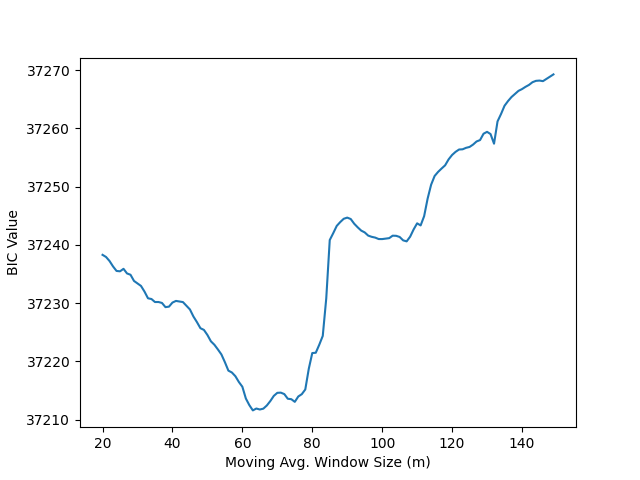
\includegraphics[width=\linewidth]{Prop_ST_Cr}
\end{subfigure}\hfill
\begin{subfigure}[!ht]{0.45\textwidth}
    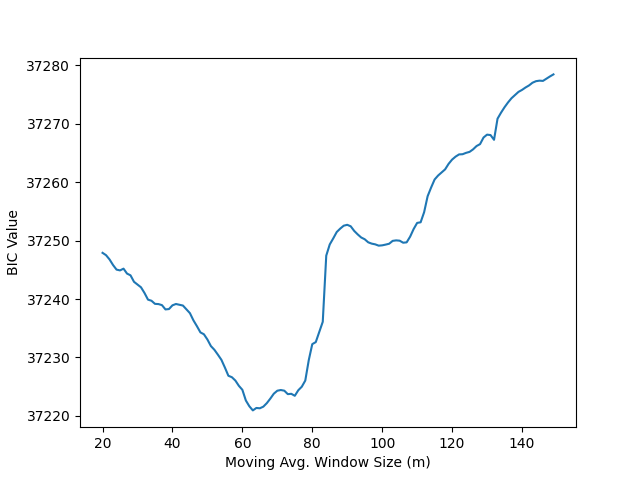
\includegraphics[width=\linewidth]{ST_Cr}
  \end{subfigure}

  \begin{subfigure}[!ht]{0.45\textwidth}
    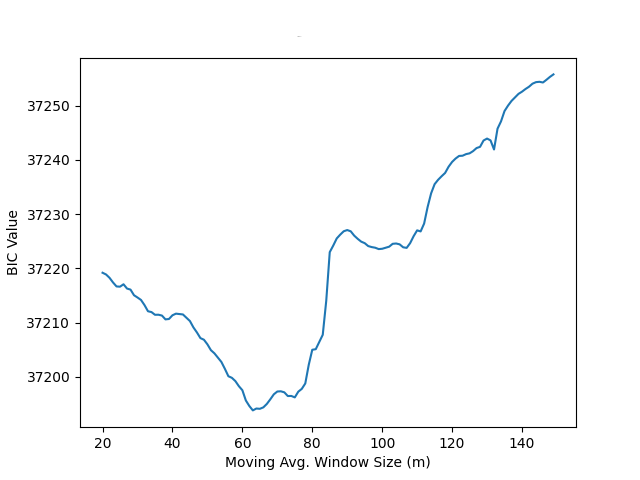
\includegraphics[width=\linewidth]{Prop_LT_Cr}
  \end{subfigure}\hfill
  \begin{subfigure}[!ht]{0.45\textwidth}
    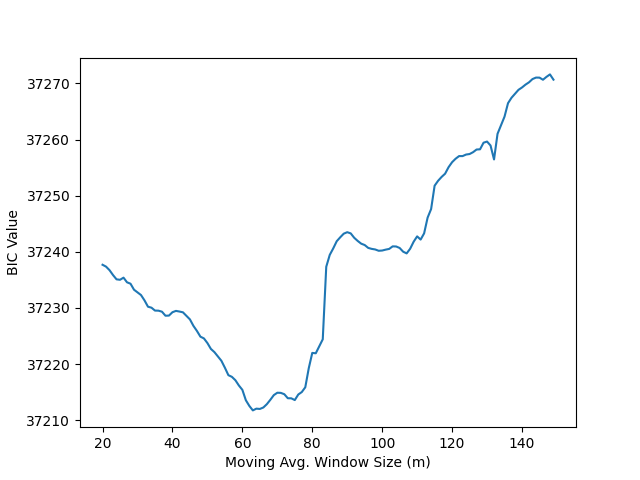
\includegraphics[width=\linewidth]{LT_Cr}
  \end{subfigure}

  \begin{subfigure}[!ht]{0.45\textwidth}
    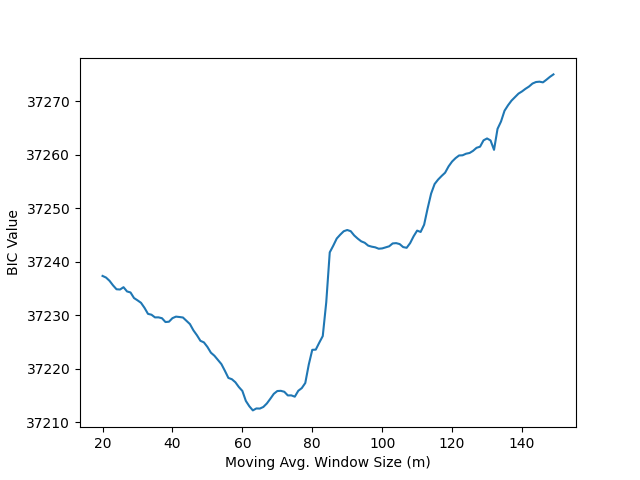
\includegraphics[width=\linewidth]{Prop_Both_Cr}
  \end{subfigure}\hfill
  \begin{subfigure}[!ht]{0.45\textwidth}
    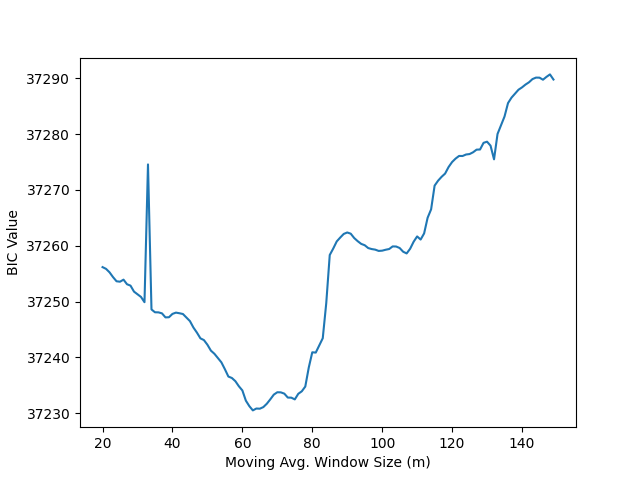
\includegraphics[width=\linewidth]{Both_Cr}
  \end{subfigure}

  \begin{subfigure}[!ht]{0.45\textwidth}
    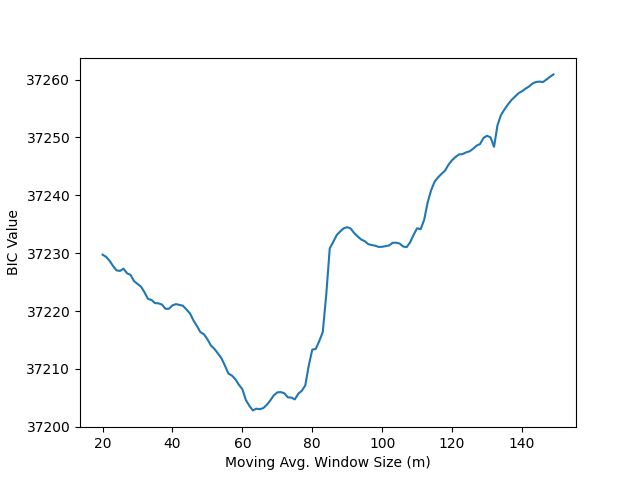
\includegraphics[width=\linewidth]{Prop_Vol_Cr}
  \end{subfigure}\hfill
  \begin{subfigure}[!ht]{0.45\textwidth}
    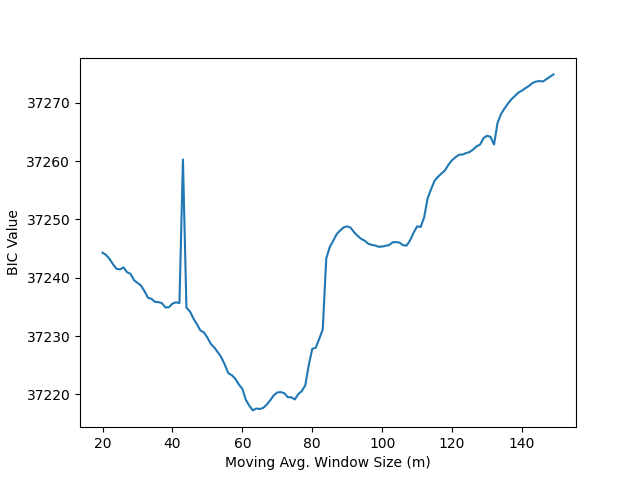
\includegraphics[width=\linewidth]{Vol_Cr}
  \end{subfigure}

\end{figure}

\newpage
%\newgeometry{a4paper, margin=3cm}
\graphicspath{{BICPlots/}}
\begin{figure}[!ht]
  \centering
  \scriptsize
  \setlength{\abovecaptionskip}{1pt}
  \setlength{\belowcaptionskip}{1pt}
  %\captionsetup{font=scriptsize}
  
  \caption[BIC Plots]{
BIC Plots. \textit{See Figure 1 notes}. This figure shows the same BIC plots for the model when the crisis indicator dummy variable is not included.}
\begin{subfigure}[!ht]{0.45\textwidth}
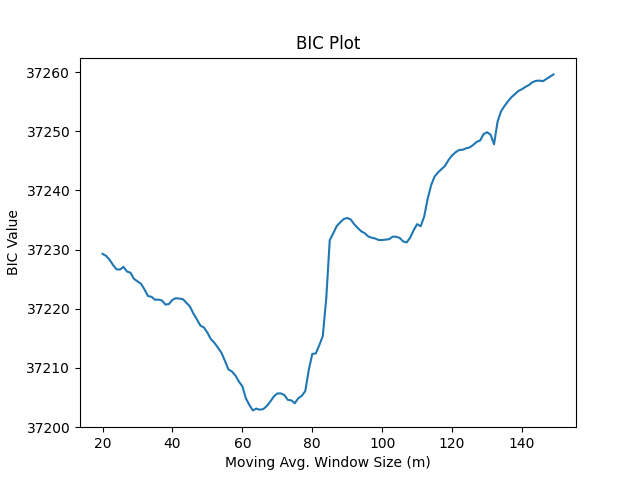
\includegraphics[width=\linewidth]{Prop_ST}
\end{subfigure}\hfill
\begin{subfigure}[!ht]{0.45\textwidth}
    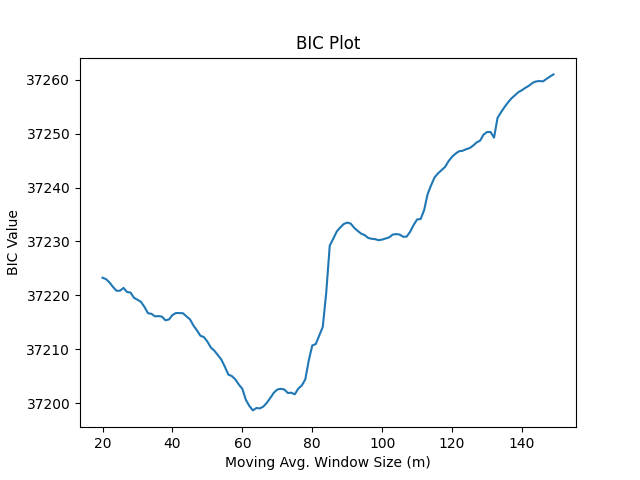
\includegraphics[width=\linewidth]{ST}
  \end{subfigure}

  \begin{subfigure}[!ht]{0.45\textwidth}
    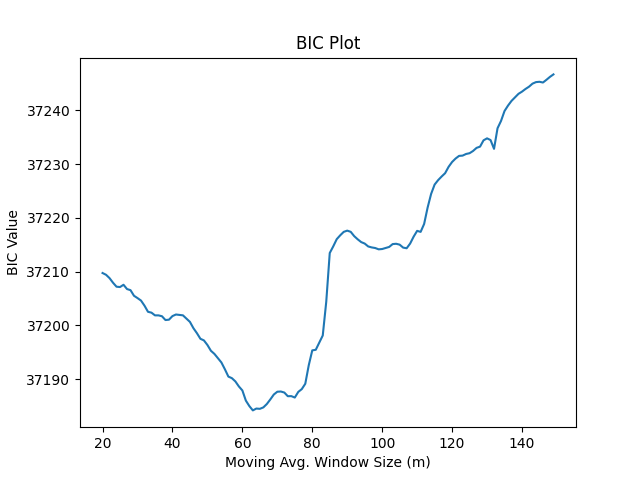
\includegraphics[width=\linewidth]{Prop_LT}
  \end{subfigure}\hfill
  \begin{subfigure}[!ht]{0.45\textwidth}
    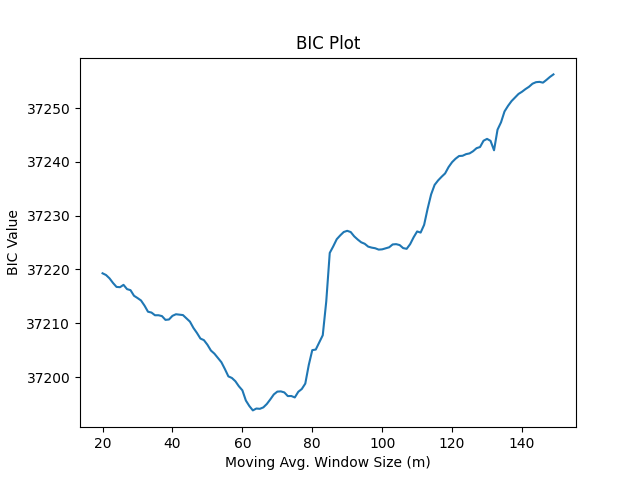
\includegraphics[width=\linewidth]{LT}
  \end{subfigure}

  \begin{subfigure}[!ht]{0.45\textwidth}
    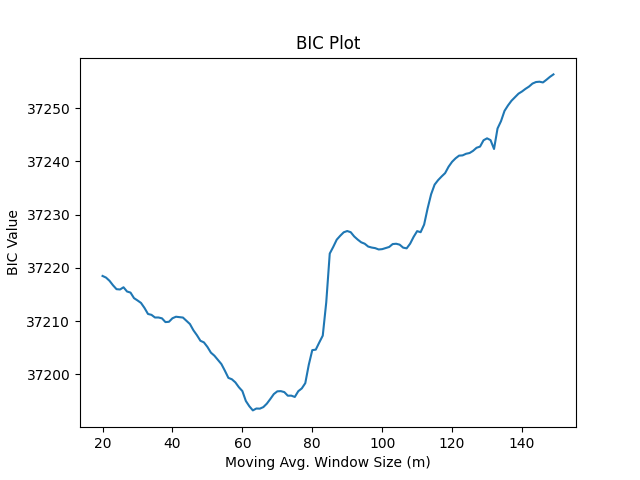
\includegraphics[width=\linewidth]{Prop_Both}
  \end{subfigure}\hfill
  \begin{subfigure}[!ht]{0.45\textwidth}
    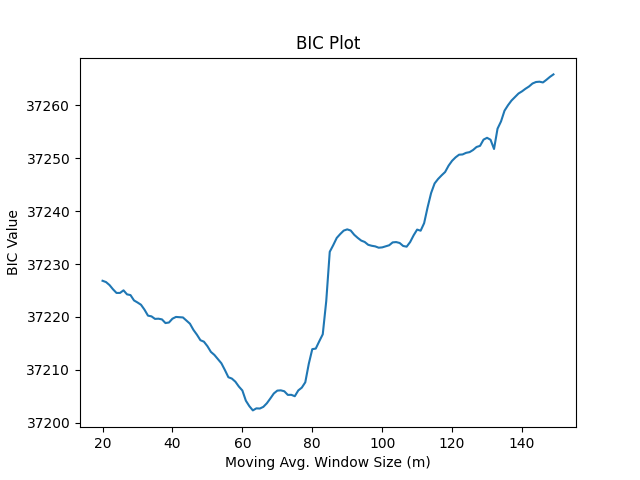
\includegraphics[width=\linewidth]{Both}
  \end{subfigure}

  \begin{subfigure}[!ht]{0.45\textwidth}
    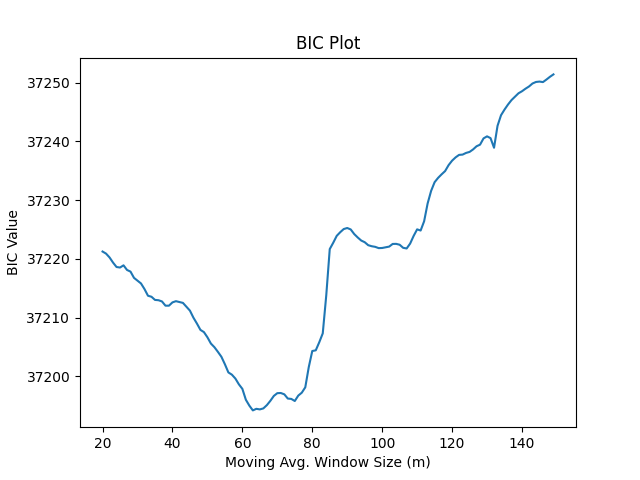
\includegraphics[width=\linewidth]{Prop_Vol}
  \end{subfigure}\hfill
  \begin{subfigure}[!ht]{0.45\textwidth}
    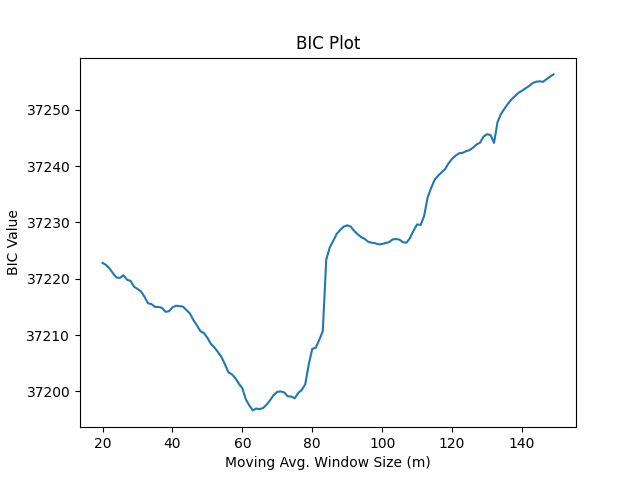
\includegraphics[width=\linewidth]{Vol}
  \end{subfigure}

\end{figure}

\pagebreak
%\restoregeometry
%\newgeometry{a4paper, margin=0.5in}
\addcontentsline{toc}{subsection}{A.2{\quad}Tables}
\section*{A.2 - Tables}
\begin{table}[!ht]
\centering
\caption{Parameter Values for Monte Carlo Simulations}
\begin{tabular}{ccccccccccc}
\midrule
\midrule
$\alpha$ & $\gamma$ & $\beta$ & $\lambda_0$ & $\lambda_1$ & $\lambda_2$ & $\delta_0$ & $\delta_{1,s}$ & $\delta_{1,l}$ & $\delta_{1}$\\
\midrule
\multicolumn{11}{c}{\textbf{Short-term component}}\\
\multicolumn{11}{l}{\textbf{Proportional}}\\
0.006 & 0.160 & 0.842 & 0.011 & 0.085 & 0.902 & - & 0.027 & - & -\\
\multicolumn{11}{l}{\textbf{Non-Proportional}}\\
0.006 & 0.160 & 0.842 & 0.011 & 0.085 & 0.902 & 0.033 & -0.003 & - & -\\
\midrule
\multicolumn{11}{c}{\textbf{Long-term component}}\\
\multicolumn{11}{l}{\textbf{Proportional}}\\
0.006 & 0.160 & 0.842 & 0.011 & 0.085 & 0.902 & - & - & 0.049  & -\\
\multicolumn{11}{l}{\textbf{Non-Proportional}}\\
0.006 & 0.160 & 0.842 & 0.011 & 0.085 & 0.902 & 0.003 & - & 0.045 & -\\
\midrule
\multicolumn{11}{c}{\textbf{Both components (additive)}}\\
\multicolumn{11}{l}{\textbf{Proportional}}\\
0.006 & 0.160 & 0.842 & 0.011 & 0.085 & 0.902 & - & -0.005 & 0.054 & -\\
\multicolumn{11}{l}{\textbf{Non-Proportional}}\\
0.006 & 0.160 & 0.842 & 0.011 & 0.085 & 0.902 & 0.008 & -0.008 & 0.046 & -\\
\midrule
\multicolumn{11}{c}{\textbf{Overall conditional variance (multiplicative)}}\\
\multicolumn{11}{l}{\textbf{Proportional}}\\
0.006 & 0.160 & 0.842 & 0.011 & 0.085 & 0.902 & - & - & - & 0.042\\
\multicolumn{11}{l}{\textbf{Non-Proportional}}\\
0.006 & 0.160 & 0.842 & 0.011 & 0.085 & 0.902 & 0.020 & - & - & 0.023\\
\midrule
\multicolumn{11}{l}{\textbf{Notes:} This table presents the "true" parameter values I used in Monte Carlo}\\
\multicolumn{11}{l}{simulations of daily market premium data. The MF2-GARCH-in-mean model}\\
\multicolumn{11}{l}{is fitted $R=1,000$ times on these simulated samples, each of size $T=15,120$.}\\
\multicolumn{11}{l}{This is repeated for the proportional and non-proportional variant of every}\\
\multicolumn{11}{l}{specification. These values were chosen based on estimates from real data \textit{(see}}\\
\multicolumn{11}{l}{\textit{Table 4 below).}}\\
\midrule
\midrule
\end{tabular}
\end{table}

\begin{table}[!ht]
\centering
\caption{Summary Statistics - Daily Market Premia}
\begin{tabular}{cccccccc}
\midrule
\midrule
\mbox{} & mean & sd & skew & kurtosis & min & max & AC(1)\\
\midrule
$r_t$ & 0.028 & 1.028 & -0.487 & 15.564 & -17.440 & 11.360 & 0.016\\
\midrule
\multicolumn{8}{l}{\textbf{Notes:} This table shows summary statistics for the U.S. daily}\\
\multicolumn{8}{l}{market premium data. The data runs from January 1964 to April}\\
\multicolumn{8}{l}{2025. The columns present the mean, standard deviation (sd),}\\
\multicolumn{8}{l}{skewness, kurtosis, minimum (min), maximum (max) and the}\\
\multicolumn{8}{l}{first-order autocorrelation coefficient (AC(1)).}\\
\midrule
\midrule
\end{tabular}
\end{table}

\begin{table}[!ht]
\centering
\caption{NBER Recession Periods}
\begin{tabular}{ccl}
\midrule
\midrule
Start date & End date & Remarks\\
\midrule
December 1969 & November 1970 & - \\
November 1973 & March 1975 & 1973 oil crisis and stagflation \\
January 1980 & July 1980 & Volcker recession I \\
July 1981 & November 1982 & Volcker recession II \\
July 1990 & March 1991 & - \\
March 2001 & November 2001 & Dot-com bubble \\
December 2007 & June 2009 & Global financial crisis \\
February 2020 & April 2020 & COVID-19 pandemic \\
\midrule
\multicolumn{3}{l}{\textbf{Notes:} This table shows the start and end dates of recession}\\
\multicolumn{3}{l}{periods defined by the U.S. National Bureau of Economic}\\
\multicolumn{3}{l}{Research (NBER) which fall within the sample period on which}\\
\multicolumn{3}{l}{the MF2-GARCH-in-mean model is estimated. The dummy}\\
\multicolumn{3}{l}{variable used to control for periods of crisis is given the value 1}\\
\multicolumn{3}{l}{for the above periods and 0 otherwise.}\\
\midrule
\midrule
\end{tabular}
\end{table}

\pagebreak
\restoregeometry
\newgeometry{a4paper, margin=0.5in}

\begin{sidewaystable}[!ht]
\centering
\scriptsize
\setlength{\tabcolsep}{3pt} 
\renewcommand{\arraystretch}{0.8}
\caption{Combined Specification Parameter Estimates (Controlling for Crisis Periods)}
\resizebox{\textwidth}{!}{
  \begin{tabular}{ccccccccccccccccc}
    \toprule\toprule
    $\alpha$ & $\gamma$ & $\beta$ & $\lambda_0$ & $\lambda_1$ & $\lambda_2$ & $\delta_0$ & $\delta_{1,s}$ & $\delta_{1,l}$ & $\delta_{1}$ & $\theta_0$ & $\theta_{1,s}$ & $\theta_{1,l}$ & $\theta_{1}$ & LLF & BIC \\
    \midrule
    \multicolumn{17}{c}{\textbf{Panel A: Short-term component}}\\
    \multicolumn{17}{l}{\textbf{Proportional}}\\
    \begin{tabular}[t]{@{}c@{}}0.007 \\ (0.014)\end{tabular} &
    \begin{tabular}[t]{@{}c@{}}0.158*** \\ (0.019)\end{tabular} &
    \begin{tabular}[t]{@{}c@{}}0.841*** \\ (0.018)\end{tabular} &
    \begin{tabular}[t]{@{}c@{}}0.012 \\ (0.020)\end{tabular} &
    \begin{tabular}[t]{@{}c@{}}0.086 \\ (0.150)\end{tabular} &
    \begin{tabular}[t]{@{}c@{}}0.900*** \\ (0.173)\end{tabular} &
    - &
    \begin{tabular}[t]{@{}c@{}}0.027** \\ (0.011)\end{tabular} &
    - & - & - &
    \begin{tabular}[t]{@{}c@{}}-0.013 \\ (0.020)\end{tabular} &
    - & - & -18567 & 37212 \\
    \multicolumn{17}{l}{\textbf{Non‑Proportional}}\\
    \begin{tabular}[t]{@{}c@{}}0.005* \\ (0.003)\end{tabular} &
    \begin{tabular}[t]{@{}c@{}}0.166*** \\ (0.015)\end{tabular} &
    \begin{tabular}[t]{@{}c@{}}0.845*** \\ (0.012)\end{tabular} &
    \begin{tabular}[t]{@{}c@{}}0.011*** \\ (0.002)\end{tabular} &
    \begin{tabular}[t]{@{}c@{}}0.081*** \\ (0.018)\end{tabular} &
    \begin{tabular}[t]{@{}c@{}}0.907*** \\ (0.018)\end{tabular} &
    \begin{tabular}[t]{@{}c@{}}0.033*** \\ (0.007)\end{tabular} &
    \begin{tabular}[t]{@{}c@{}}-0.003*** \\ (0.001)\end{tabular} &
    - & - &
    \begin{tabular}[t]{@{}c@{}}0.009 \\ (0.008)\end{tabular} &
    \begin{tabular}[t]{@{}c@{}}-0.009 \\ (0.009)\end{tabular} &
    - & - & -18562 & 37221 \\
    \multicolumn{17}{l}{LRT: 9.928***}\\
    \midrule

    \multicolumn{17}{c}{\textbf{Panel B: Long-term component}}\\
    \multicolumn{17}{l}{\textbf{Proportional}}\\
    \begin{tabular}[t]{@{}c@{}}0.006** \\ (0.003)\end{tabular} &
    \begin{tabular}[t]{@{}c@{}}0.160*** \\ (0.015)\end{tabular} &
    \begin{tabular}[t]{@{}c@{}}0.842*** \\ (0.013)\end{tabular} &
    \begin{tabular}[t]{@{}c@{}}0.011*** \\ (0.003)\end{tabular} &
    \begin{tabular}[t]{@{}c@{}}0.085*** \\ (0.018)\end{tabular} &
    \begin{tabular}[t]{@{}c@{}}0.902*** \\ (0.020)\end{tabular} &
    - & - &
    \begin{tabular}[t]{@{}c@{}}0.049*** \\ (0.009)\end{tabular} &
    - & - & - &
    \begin{tabular}[t]{@{}c@{}}-0.002*** \\ (0.001)\end{tabular} &
    - & -18558 & \textbf{37194} \\
    \multicolumn{17}{l}{\textbf{Non‑Proportional}}\\
    \begin{tabular}[t]{@{}c@{}}0.006* \\ (0.004)\end{tabular} &
    \begin{tabular}[t]{@{}c@{}}0.161*** \\ (0.015)\end{tabular} &
    \begin{tabular}[t]{@{}c@{}}0.843*** \\ (0.014)\end{tabular} &
    \begin{tabular}[t]{@{}c@{}}0.011* \\ (0.006)\end{tabular} &
    \begin{tabular}[t]{@{}c@{}}0.080*** \\ (0.030)\end{tabular} &
    \begin{tabular}[t]{@{}c@{}}0.907*** \\ (0.036)\end{tabular} &
    \begin{tabular}[t]{@{}c@{}}0.003 \\ (0.003)\end{tabular} &
    - &
    \begin{tabular}[t]{@{}c@{}}0.045*** \\ (0.017)\end{tabular} &
    - &
    \begin{tabular}[t]{@{}c@{}}-0.054 \\ (0.060)\end{tabular} &
    - &
    \begin{tabular}[t]{@{}c@{}}0.049 \\ (0.049)\end{tabular} &
    - & -18558 & 37212 \\
    \multicolumn{17}{l}{LRT: 1.358}\\
    \midrule

    \multicolumn{17}{c}{\textbf{Panel C: Both components (additive)}}\\
    \multicolumn{17}{l}{\textbf{Proportional}}\\
    \begin{tabular}[t]{@{}c@{}}0.006 \\ (0.013)\end{tabular} &
    \begin{tabular}[t]{@{}c@{}}0.161*** \\ (0.015)\end{tabular} &
    \begin{tabular}[t]{@{}c@{}}0.844*** \\ (0.016)\end{tabular} &
    \begin{tabular}[t]{@{}c@{}}0.012* \\ (0.006)\end{tabular} &
    \begin{tabular}[t]{@{}c@{}}0.085** \\ (0.035)\end{tabular} &
    \begin{tabular}[t]{@{}c@{}}0.901*** \\ (0.042)\end{tabular} &
    - &
    \begin{tabular}[t]{@{}c@{}}-0.005 \\ (0.021)\end{tabular} &
    \begin{tabular}[t]{@{}c@{}}0.054** \\ (0.023)\end{tabular} &
    - & - &
    \begin{tabular}[t]{@{}c@{}}-0.012** \\ (0.006)\end{tabular} &
    \begin{tabular}[t]{@{}c@{}}0.009 \\ (0.012)\end{tabular} &
    - & -18558 & 37212 \\
    \multicolumn{17}{l}{\textbf{Non‑Proportional}}\\
    \begin{tabular}[t]{@{}c@{}}0.006 \\ (0.003)\end{tabular} &
    \begin{tabular}[t]{@{}c@{}}0.162*** \\ (0.016)\end{tabular} &
    \begin{tabular}[t]{@{}c@{}}0.844*** \\ (0.014)\end{tabular} &
    \begin{tabular}[t]{@{}c@{}}0.011 \\ (0.007)\end{tabular} &
    \begin{tabular}[t]{@{}c@{}}0.081** \\ (0.036)\end{tabular} &
    \begin{tabular}[t]{@{}c@{}}0.906*** \\ (0.043)\end{tabular} &
    \begin{tabular}[t]{@{}c@{}}0.008 \\ (0.006)\end{tabular} &
    \begin{tabular}[t]{@{}c@{}}-0.008 \\ (0.007)\end{tabular} &
    \begin{tabular}[t]{@{}c@{}}0.046*** \\ (0.012)\end{tabular} &
    - &
    \begin{tabular}[t]{@{}c@{}}-0.050 \\ (0.067)\end{tabular} &
    \begin{tabular}[t]{@{}c@{}}-0.002 \\ (0.002)\end{tabular} &
    \begin{tabular}[t]{@{}c@{}}0.048 \\ (0.041)\end{tabular} &
    - & -18557 & 37230 \\
    \multicolumn{17}{l}{LRT: 0.990}\\
    \midrule

    \multicolumn{17}{c}{\textbf{Panel D: Overall conditional variance (multiplicative)}}\\
    \multicolumn{17}{l}{\textbf{Proportional}}\\
    \begin{tabular}[t]{@{}c@{}}0.007 \\ (0.009)\end{tabular} &
    \begin{tabular}[t]{@{}c@{}}0.158*** \\ (0.016)\end{tabular} &
    \begin{tabular}[t]{@{}c@{}}0.839*** \\ (0.014)\end{tabular} &
    \begin{tabular}[t]{@{}c@{}}0.011** \\ (0.005)\end{tabular} &
    \begin{tabular}[t]{@{}c@{}}0.080*** \\ (0.031)\end{tabular} &
    \begin{tabular}[t]{@{}c@{}}0.907*** \\ (0.035)\end{tabular} &
    - & - & - &
    \begin{tabular}[t]{@{}c@{}}0.042*** \\ (0.010)\end{tabular} &
    - & - & - &
    \begin{tabular}[t]{@{}c@{}}-0.014* \\ (0.008)\end{tabular} &
    -18563 & 37203 \\
    \multicolumn{17}{l}{\textbf{Non‑Proportional}}\\
    \begin{tabular}[t]{@{}c@{}}0.006 \\ (0.012)\end{tabular} &
    \begin{tabular}[t]{@{}c@{}}0.162*** \\ (0.025)\end{tabular} &
    \begin{tabular}[t]{@{}c@{}}0.841*** \\ (0.018)\end{tabular} &
    \begin{tabular}[t]{@{}c@{}}0.011 \\ (0.016)\end{tabular} &
    \begin{tabular}[t]{@{}c@{}}0.080 \\ (0.084)\end{tabular} &
    \begin{tabular}[t]{@{}c@{}}0.908*** \\ (0.101)\end{tabular} &
    \begin{tabular}[t]{@{}c@{}}0.020 \\ (0.059)\end{tabular} &
    - & - &
    \begin{tabular}[t]{@{}c@{}}0.023 \\ (0.083)\end{tabular} &
    \begin{tabular}[t]{@{}c@{}}-0.005 \\ (0.016)\end{tabular} &
    - & - &
    \begin{tabular}[t]{@{}c@{}}-0.004 \\ (0.022)\end{tabular} &
    -18560 & 37217 \\
    \multicolumn{17}{l}{LRT: 4.850*}\\
    \midrule
\multicolumn{17}{l}{\textbf{Notes:} This table shows the results of the QMLE parameter estimates for the MF2-GARCH-in-mean model. The numbers in parentheses are Bollerslev-}\\
\multicolumn{17}{l}{Wooldridge robust standard errors. *** ,** and * indicate significance at the 1\%, 5\% and 10\% level. Each panel shows the results for a different}\\
\multicolumn{17}{l}{specification, depending on which components of volatility are included. Each panel shows the proportional (no intercept) and non-proportional}\\
\multicolumn{17}{l}{variant. The likelihood ratio test (LRT) statistic for the proportional variant against the non-proportional variant is also shown at the bottom of each}\\
\multicolumn{17}{l}{panel. All specifications are estimated using daily U.S. market premium data for the period January 1964 to April 2025 inclusive. The moving average}\\
\multicolumn{17}{l}{window size (m) which minmizes the Bayesian Information Criterion for all specifications is m=63.}\\
\midrule
\midrule
  \end{tabular}%
}
\end{sidewaystable}

\pagebreak
\restoregeometry
\newgeometry{a4paper, margin=0.5in}

\begin{table}[!ht]
\centering
\setlength{\tabcolsep}{3pt} 
\caption{Combined Specification Parameter Estimates (\textbf{Not} Controlling for Crisis Periods)}
\resizebox{\textwidth}{!}{
  \begin{tabular}{ccccccccccccc}
    \toprule\toprule
    $\alpha$ & $\gamma$ & $\beta$ & $\lambda_0$ & $\lambda_1$ & $\lambda_2$ & $\delta_0$ & $\delta_{1,s}$ & $\delta_{1,l}$ & $\delta_{1}$ & LLF & BIC \\
    \midrule
    \multicolumn{13}{c}{\textbf{Panel A: Short-term component}}\\
    \multicolumn{13}{l}{\textbf{Proportional}}\\
    \begin{tabular}[t]{@{}c@{}}0.007* \\ (0.004)\end{tabular} &
    \begin{tabular}[t]{@{}c@{}}0.158*** \\ (0.015)\end{tabular} &
    \begin{tabular}[t]{@{}c@{}}0.840*** \\ (0.013)\end{tabular} &
    \begin{tabular}[t]{@{}c@{}}0.012 \\ (0.011)\end{tabular} &
    \begin{tabular}[t]{@{}c@{}}0.086 \\ (0.066)\end{tabular} &
    \begin{tabular}[t]{@{}c@{}}0.901*** \\ (0.079)\end{tabular} &
    - &
    \begin{tabular}[t]{@{}c@{}}0.024** \\ (0.010)\end{tabular} &
    - & - &
    -18568 & 37203 \\
    \multicolumn{13}{l}{\textbf{Non‑Proportional}}\\
    \begin{tabular}[t]{@{}c@{}}0.006*** \\ (0.002)\end{tabular} &
    \begin{tabular}[t]{@{}c@{}}0.163*** \\ (0.015)\end{tabular} &
    \begin{tabular}[t]{@{}c@{}}0.843*** \\ (0.014)\end{tabular} &
    \begin{tabular}[t]{@{}c@{}}0.011*** \\ (0.003)\end{tabular} &
    \begin{tabular}[t]{@{}c@{}}0.089*** \\ (0.027)\end{tabular} &
    \begin{tabular}[t]{@{}c@{}}0.898*** \\ (0.029)\end{tabular} &
    \begin{tabular}[t]{@{}c@{}}0.043*** \\ (0.007)\end{tabular} &
    \begin{tabular}[t]{@{}c@{}}-0.013** \\ (0.005)\end{tabular} &
    - & - &
    -18561 & 37199 \\
    \multicolumn{13}{l}{LRT: 13.806***}\\
    \midrule

    \multicolumn{13}{c}{\textbf{Panel B: Long-term component}}\\
    \multicolumn{13}{l}{\textbf{Proportional}}\\
    \begin{tabular}[t]{@{}c@{}}0.006** \\ (0.003)\end{tabular} &
    \begin{tabular}[t]{@{}c@{}}0.160*** \\ (0.015)\end{tabular} &
    \begin{tabular}[t]{@{}c@{}}0.842*** \\ (0.013)\end{tabular} &
    \begin{tabular}[t]{@{}c@{}}0.011*** \\ (0.003)\end{tabular} &
    \begin{tabular}[t]{@{}c@{}}0.084*** \\ (0.021)\end{tabular} &
    \begin{tabular}[t]{@{}c@{}}0.902*** \\ (0.022)\end{tabular} &
    - & - &
    \begin{tabular}[t]{@{}c@{}}0.049*** \\ (0.010)\end{tabular} &
    - &
    -18558 & 37184 \\
    \multicolumn{13}{l}{\textbf{Non‑Proportional}}\\
    \begin{tabular}[t]{@{}c@{}}0.006 \\ (0.033)\end{tabular} &
    \begin{tabular}[t]{@{}c@{}}0.160*** \\ (0.021)\end{tabular} &
    \begin{tabular}[t]{@{}c@{}}0.843*** \\ (0.020)\end{tabular} &
    \begin{tabular}[t]{@{}c@{}}0.011 \\ (0.020)\end{tabular} &
    \begin{tabular}[t]{@{}c@{}}0.085 \\ (0.329)\end{tabular} &
    \begin{tabular}[t]{@{}c@{}}0.902** \\ (0.386)\end{tabular} &
    \begin{tabular}[t]{@{}c@{}}0.003 \\ (0.009)\end{tabular} &
    - & 
    \begin{tabular}[t]{@{}c@{}}0.046 \\ (0.038)\end{tabular} &
    - &
    -18558 & 37194 \\
    \multicolumn{13}{l}{LRT: 0.034}\\
    \midrule

    \multicolumn{13}{c}{\textbf{Panel C: Both components (additive)}}\\
    \multicolumn{13}{l}{\textbf{Proportional}}\\
    \begin{tabular}[t]{@{}c@{}}0.006* \\ (0.003)\end{tabular} &
    \begin{tabular}[t]{@{}c@{}}0.161*** \\ (0.015)\end{tabular} &
    \begin{tabular}[t]{@{}c@{}}0.843*** \\ (0.013)\end{tabular} &
    \begin{tabular}[t]{@{}c@{}}0.012*** \\ (0.003)\end{tabular} &
    \begin{tabular}[t]{@{}c@{}}0.085*** \\ (0.023)\end{tabular} &
    \begin{tabular}[t]{@{}c@{}}0.901*** \\ (0.024)\end{tabular} &
    - &
    \begin{tabular}[t]{@{}c@{}}-0.008 \\ (0.008)\end{tabular} &
    \begin{tabular}[t]{@{}c@{}}0.057*** \\ (0.015)\end{tabular} &
    - &
    -18558 & 37193 \\
    \multicolumn{13}{l}{\textbf{Non-Proportional}}\\
    \begin{tabular}[t]{@{}c@{}}0.005 \\ (0.033)\end{tabular} &
    \begin{tabular}[t]{@{}c@{}}0.162*** \\ (0.021)\end{tabular} &
    \begin{tabular}[t]{@{}c@{}}0.843*** \\ (0.030)\end{tabular} &
    \begin{tabular}[t]{@{}c@{}}0.012 \\ (0.039)\end{tabular} &
    \begin{tabular}[t]{@{}c@{}}0.088 \\ (0.139)\end{tabular} &
    \begin{tabular}[t]{@{}c@{}}0.898*** \\ (0.188)\end{tabular} &
    \begin{tabular}[t]{@{}c@{}}0.013 \\ (0.138)\end{tabular} &
    \begin{tabular}[t]{@{}c@{}}-0.013 \\ (0.104)\end{tabular} &
    \begin{tabular}[t]{@{}c@{}}0.046 \\ (0.332)\end{tabular} &
    - &
    -18558 & 37202 \\
    \multicolumn{13}{l}{LRT: 0.542}\\
    \midrule

    \multicolumn{13}{c}{\textbf{Panel D: Overall conditional variance (multiplicative)}}\\
    \multicolumn{13}{l}{\textbf{Proportional}}\\
    \begin{tabular}[t]{@{}c@{}}0.007 \\ (0.005)\end{tabular} &
    \begin{tabular}[t]{@{}c@{}}0.158*** \\ (0.015)\end{tabular} &
    \begin{tabular}[t]{@{}c@{}}0.839*** \\ (0.013)\end{tabular} &
    \begin{tabular}[t]{@{}c@{}}0.010*** \\ (0.003)\end{tabular} &
    \begin{tabular}[t]{@{}c@{}}0.079*** \\ (0.023)\end{tabular} &
    \begin{tabular}[t]{@{}c@{}}0.909*** \\ (0.024)\end{tabular} &
    - & - & - &
    \begin{tabular}[t]{@{}c@{}}0.037*** \\ (0.007)\end{tabular} &
    -18563 & 37194 \\
    \multicolumn{13}{l}{\textbf{Non‑Proportional}}\\
    \begin{tabular}[t]{@{}c@{}}0.007 \\ (0.013)\end{tabular} &
    \begin{tabular}[t]{@{}c@{}}0.159*** \\ (0.016)\end{tabular} &
    \begin{tabular}[t]{@{}c@{}}0.840*** \\ (0.022)\end{tabular} &
    \begin{tabular}[t]{@{}c@{}}0.011** \\ (0.005)\end{tabular} &
    \begin{tabular}[t]{@{}c@{}}0.083** \\ (0.034)\end{tabular} &
    \begin{tabular}[t]{@{}c@{}}0.904*** \\ (0.039)\end{tabular} &
    \begin{tabular}[t]{@{}c@{}}0.022 \\ (0.015)\end{tabular} &
    - & - &
    \begin{tabular}[t]{@{}c@{}}0.019 \\ (0.034)\end{tabular} &
    -18560 & 37197 \\
    \multicolumn{13}{l}{LRT: 7.182**}\\
    \midrule
\multicolumn{13}{l}{\textbf{Notes: }\textit{See Table 4 notes.} This table show parameter estimates when the crisis dummy variable is not included.}\\
\midrule
\midrule
  \end{tabular}%
}
\end{table}

\pagebreak
\restoregeometry
%\newgeometry{a4paper, margin=0.2in}
\begin{table}[!ht]
\centering
\caption{Summary Statistics - With Crisis Control Dummy}
\begin{tabular}{ccccc}
\multicolumn{5}{c}{(Proportional LT Component Specification)}\\
\midrule
\midrule
\mbox{} & mean & min & max & AC(1)\\
\midrule
\mbox{$\sigma^2_t$}& 1.051 & 0.122 & 60.992 & 0.94736\\
\mbox{$h_t$} & 1.186 & 0.474 & 69.731 & 0.98251\\
\mbox{$\tau_t$} & 0.830 & 0.236 & 3.810 & 0.99988\\
\midrule
\multicolumn{5}{l}{\textbf{Notes:} This table shows summary statistics}\\
\multicolumn{5}{l}{for the daily conditional variance and its}\\
\multicolumn{5}{l}{components as estimated by MF2-GARCH}\\
\multicolumn{5}{l}{in the proportional (no intercept) long-}\\
\multicolumn{5}{l}{term component specification when}\\
\multicolumn{5}{l}{controlling for crisis periods. The columns}\\
\multicolumn{5}{l}{show the mean, maximum (max), minimum}\\
\multicolumn{5}{l}{(min)and the first-order autocorrelation}\\
\multicolumn{5}{l}{coefficient (AR(1)).}\\
\midrule
\end{tabular}
\end{table}

\begin{table}[!ht]
\centering
\caption{Summary Statistics - Without Crisis Control Dummy}
\begin{tabular}{ccccc}
\multicolumn{5}{c}{(Proportional LT Component Specification)}\\
\midrule
\midrule
\mbox{} & mean & min & max & AC(1)\\
\midrule
\mbox{$\sigma^2_t$}& 1.051 & 0.122 & 60.969 & 0.94738\\
\mbox{$h_t$} & 1.186 & 0.474 & 69.720 & 0.92859\\
\mbox{$\tau_t$} & 0.830 & 0.236 & 3.793 & 0.99988\\
\midrule
\multicolumn{5}{l}{\textbf{Notes:} \textit{See Table 6 notes.} This table}\\
\multicolumn{5}{l}{presents the summary statistics for the}\\
\multicolumn{5}{l}{proportional long-term component}\\
\multicolumn{5}{l}{specification without controlling for}\\
\multicolumn{5}{l}{crisis periods.}\\
\midrule
\midrule
\end{tabular}
\end{table}

\pagebreak
\newgeometry{a4paper, margin=0.5in}
\begin{table}[!ht]
  \centering
  \scriptsize
  \setlength\tabcolsep{3pt}
  \caption{Monte Carlo Parameter Estimates \& Standard Deviations}
  \resizebox{\linewidth}{!}{
    \begin{tabular}{lccccccccccc}
      \toprule
      & $\alpha$ & $\gamma$ & $\beta$ & $\lambda_0$ & $\lambda_1$ & $\lambda_2$ 
      & $\delta_0$ & $\delta_{1,s}$ & $\delta_{1,l}$ & $\delta_{1}$\\
      \midrule
      \multicolumn{12}{c}{\textbf{Short-term component}}\\
      \multicolumn{12}{l}{\textbf{Proportional}}\\
      True & 0.00600 & 0.16000 & 0.84200 & 0.01100 & 0.08500 & 0.90200 & - & 0.02700 & - & -\\
      Bias & -0.00116 & -0.00128 & 0.00198 & 0.00082 & 0.00119 & -0.00226 & - & -0.00011 & - & -\\
      (\%)  & (-19.33\%) & (-0.80\%) & (0.24\%) & (7.45\%) & (1.40\%) & (-0.25\%) & - & (-0.41\%) & - & -\\
      S.d.  & 0.00353 & 0.00684 & 0.00675 & 0.00601 & 0.03777 & 0.04460 & - & 0.00468 & - & -\\
      \addlinespace
      \multicolumn{12}{l}{\textbf{Non-Proportional}}\\
      True & 0.00600 & 0.16000 & 0.84200 & 0.01100 & 0.08500 & 0.90200 & 0.03300 & -0.00300 & - & -\\
      Bias & -0.00115 & -0.00072 & 0.00122 & 0.00086 & 0.00147 & -0.00259 & -0.00155 & 0.00150 & - & -\\
      (\%)  & (-19.17\%) & (-0.45\%) & (0.14\%) & (7.82\%) & (1.73\%) & (-0.29\%) & (-4.70\%) & (-50.00\%) & - & -\\
      S.d.  & 0.00356 & 0.00691 & 0.00711 & 0.00603 & 0.03789 & 0.04476 & 0.01192 & 0.01303 & - & -\\
      \midrule
      \multicolumn{12}{c}{\textbf{Long-term component}}\\
      \multicolumn{12}{l}{\textbf{Proportional}}\\
      True & 0.00600 & 0.16000 & 0.84200 & 0.01100 & 0.08500 & 0.90200 & - & - & 0.04900 & -\\
      Bias & -0.00116 & -0.00070 & 0.00139 & 0.00071 & 0.00052 & -0.00145 & - & - & -0.00010 & -\\
      (\%)  & (-19.33\%) & (-0.44\%) & (0.17\%) & (6.45\%) & (0.61\%) & (-0.16\%) & - & - & (-0.20\%) & -\\
      S.d.  & 0.00353 & 0.00693 & 0.00678 & 0.00578 & 0.03593 & 0.04253 & - & - & 0.00636 & -\\
      \addlinespace
      \multicolumn{12}{l}{\textbf{Non-Proportional}}\\
      True & 0.00600 & 0.16000 & 0.84200 & 0.01100 & 0.08500 & 0.90200 & 0.00300 & - & 0.04500 & -\\
      Bias & -0.00116 & -0.00070 & 0.00140 & 0.00073 & 0.00075 & -0.00170 & -0.00035 & - & 0.00022 & -\\
      (\%)  & (-19.33\%) & (-0.44\%) & (0.17\%) & (6.64\%) & (0.88\%) & (-0.19\%) & (-11.67\%) & - & (0.49\%) & -\\
      S.d.  & 0.00355 & 0.00692 & 0.00679 & 0.00577 & 0.03660 & 0.04314 & 0.01413 & - & 0.01833 & -\\
      \midrule
      \multicolumn{12}{c}{\textbf{Both components (additive)}}\\
      \multicolumn{12}{l}{\textbf{Proportional}}\\
      True & 0.00600 & 0.16000 & 0.84200 & 0.01100 & 0.08500 & 0.90200 & - & -0.00500 & 0.05400 & -\\
      Bias & -0.00116 & -0.00064 & 0.00124 & 0.00066 & 0.00050 & -0.00138 & - & 0.00057 & -0.00079 & -\\
      (\%)  & (-19.33\%) & (-0.40\%) & (0.15\%) & (6.00\%) & (0.59\%) & (-0.15\%) & - & (-11.40\%) & (-1.46\%) & -\\
      S.d.  & 0.00354 & 0.00692 & 0.00702 & 0.00563 & 0.03599 & 0.04239 & - & 0.01071 & 0.01272 & -\\
      \addlinespace
      \multicolumn{12}{l}{\textbf{Non-Proportional}}\\
      True & 0.00600 & 0.16000 & 0.84200 & 0.01100 & 0.08500 & 0.90200 & 0.00800 & -0.00800 & 0.04600 & -\\
      Bias & -0.00115 & -0.00061 & 0.00108 & 0.00068 & 0.00054 & -0.00145 & -0.00166 & 0.00156 & 0.00010 & -\\
      (\%)  & (-19.17\%) & (-0.38\%) & (0.13\%) & (6.18\%) & (0.64\%) & (-0.16\%) & (-20.75\%) & (-19.50\%) & (0.22\%) & -\\
      S.d.  & 0.00356 & 0.00693 & 0.00710 & 0.00568 & 0.03638 & 0.04281 & 0.01735 & 0.01309 & 0.01863 & -\\
      \midrule
      \multicolumn{12}{c}{\textbf{Overall conditional variance (multiplicative)}}\\
      \multicolumn{12}{l}{\textbf{Proportional}}\\
      True & 0.00600 & 0.16000 & 0.84200 & 0.01100 & 0.08500 & 0.90200 & - & - & - & 0.04200\\
      Bias & -0.00119 & -0.00144 & 0.00211 & 0.00077 & 0.00095 & -0.00195 & - & - & - & -0.00006\\
      (\%)  & (-19.83\%) & (-0.90\%) & (0.25\%) & (7.00\%) & (1.12\%) & (-0.22\%) & - & - & - & (-0.14\%)\\
      S.d.  & 0.00350 & 0.00682 & 0.00672 & 0.00594 & 0.03701 & 0.04378 & - & - & - & 0.00610\\
      \addlinespace
      \multicolumn{12}{l}{\textbf{Non-Proportional}}\\
      True & 0.00600 & 0.16000 & 0.84200 & 0.01100 & 0.08500 & 0.90200 & 0.02000 & - & - & 0.02300\\
      Bias & -0.00117 & -0.00109 & 0.00176 & 0.00081 & 0.00116 & -0.00221 & -0.00018 & - & - & 0.00011\\
      (\%)  & (-19.50\%) & (-0.68\%) & (0.21\%) & (7.36\%) & (1.36\%) & (-0.25\%) & (-0.90\%) & - & - & (0.48\%)\\
      S.d.  & 0.00353 & 0.00686 & 0.00689 & 0.00600 & 0.03745 & 0.04429 & 0.00846 & - & - & 0.01140\\
      \midrule
      \multicolumn{12}{l}{\textbf{Notes:} This table presents the results of MF2-GARCH-in-mean QMLE parameter estimation on data}\\
      \multicolumn{12}{l}{generated by Monte Carlo simulations of daily market premia. Each specification was fitted on a simulated}\\
      \multicolumn{12}{l}{sample of size $T=30,240$ and this was repeated $R=1,000$ times. The table shows the true parameter}\\
      \multicolumn{12}{l}{values (True), the average bias of the parameter estimates (value and percent), and the standard}\\
      \multicolumn{12}{l}{deviation (S.d.) of the parameter estimates across the 1,000 simulations.}\\
      \bottomrule
    \end{tabular}%
  }
\end{table}

\pagebreak
\restoregeometry
\addcontentsline{toc}{subsection}{A.3{\quad}Code}
\section*{A.3 - Code}
The full Python code and data files are provided as attachments to the digital version of this thesis. The code can also be found online at: \url{}

\end{document}